\chapter{Results}
\label{chap:3}
\ChapterPageStuff{3}

\section{Introduction}
In \Cref{sec:ch2_preamble}, the methodology was created for a web-based software system. As described in this section, a user can have multiple systems and subsystems linked to their account. The implementation is done for multiple software systems in this section. The system implementation will focus more on the development of the logging mechanism, and the critical analysis will prioritise software maintenance using a utilisation analysis.

\section{Implementation}\label{sec:ch3_implementation}
In this section, the implementation of the development of the solution will be discussed using a test system to verify it. The test system is created in a \texttt{ASP.NET Core Web SDK} software environment.

\subsection{User activity types}
In \Cref{fig:ch2_user_based_actvity_classification} the user-based clarification flow diagram uses the \Cref{tbl:ch2_requirementsForUserActivtyEvent} to identify and capture some of the log attributes. The event logs should consist of multiple cases (\ref{fr:requirementsUserBased2}) that are the primary identifiers for the event log which is the user activity types.\par Using the basic operations of the system and what users interact with the user activate types can be made for each software system. For the test system, the basic use will be:

\begin{itemize}
	\item monitor resource usage dynamic dashboards,
	\item generate \texttt{PDF} reports of the displayed data.
\end{itemize}

Reporting and monitoring are important for this test system so the user activity types will need to focus on these activity types. To satisfy the \ref{fr:requirementsUserBased2}, \ref{fr:requirementsUserBased5} and \ref{fr:requirementsUserBased6} the user actvity types is defined in \Cref{tbl:ch3_testActivityTypes}.

\begin{table}[!htb]
	\centering
	\caption[Test user activity types]{\textit{Test user activity types}}
	\label{tbl:ch3_testActivityTypes}
	\begin{tabularx}{\textwidth}{|X|l|X|}
		\hline \textbf{Activity} & \textbf{Functional requirement} & \textbf{Description} \\
		\hline \texttt{SystemAccess} & \ref{fr:uatType1} & \RaggedRight This activity type detects when a user has navigated to a certain subsystem. \\ 
		\hline \texttt{General} & \ref{fr:uatType3} & \RaggedRight This general activity type is for all other activities that the user initiates that send \textit{HTTP request} back to the server. \\
		\hline \texttt{ReportExport} & \ref{fr:uatType3} & \RaggedRight The other main function of the system is for reporting purposes. Separating this type of activity in its category to capture all report generation activities that the user has initiated. \\ 
		\hline
	\end{tabularx}
\end{table}

\Cref{tbl:ch3_testActivityTypes} doesn't contain any session changes (\ref{fr:uatType3}) user types. These activities are only triggered when the user log's into their system or terminates their session by pressing the log-out button.

\subsection{Log attibutes}\label{sec:ch3_implementationLogAtrributes}
Using the functional requirements discussed in \Cref{sec:ch2_logAttributesRequirements} data columns are made for the user-based event's log attributes. These log attributes for a structured database are defined in \Cref{tbl:ch3_Log_Attributes}. 

\begin{table}[!htb]
	\centering
	\caption[Logging attributes]
	{\textit{Logging attributes}}
	\label{tbl:ch3_Log_Attributes}
	\begin{tabularx}{\textwidth}{|l|l|X|}
		\hline \textbf{Column name} & \textbf{Requirement ID} & \textbf{Description}\\
		\hline \texttt{ID} & \ref{fr:lpa1} & User based actvity primary identifier. \\
		\hline \texttt{TimeStamp} & \ref{fr:lpa2} & Date timesstamp when the activity has occur. \\
		\hline \texttt{ActivityType} & \ref{fr:lpa3} & Activity type of the log event. \\
		\hline \texttt{UserId} & \ref{fr:lpa4} & Identification number of the user associated with the log event. \\
		\hline \texttt{SystemId} & \ref{fr:lpa5} & System where the activity has occur. \\
		\hline \texttt{SubsystemId} & \ref{fr:lpa5} & Subsystem where the activity has occur. \\
		\hline \texttt{MetaData} & \ref{fr:lpa6} & Metadata captured from the \textit{HTTP request}. \\
		\hline \texttt{ClientId} & \ref{fr:lpa7} & Additional identifiers for the log event. In this case different configurations of the same system for a specific client. \\
		\hline
	\end{tabularx}
\end{table}

The data columns in \Cref{tbl:ch3_Log_Attributes} are used in a structured database. The test that is used is a \texttt{MySQL} database. This database has pre-existing tables that expand on other data such as the \texttt{UserId}, \texttt{SystemId} and \texttt{SubSystemId}. For the \texttt{MetaData} the \texttt{JSON} is similar to \Cref{fig:ch3_MetadataJson}.

\medskip

\begin{lstlisting}[style=json, caption={\textit{Metadata JSON}}, label={fig:ch3_MetadataJson}] 
	{
		"RequestOrigin": "/System/Subsystem1/GetData",
		"RequestElementID": "ButtonSaveCsv",
		"RequestParameters": {
			"tagIds": [
				"6284",
				"20320"
			],
			"toDate": "2020-04-06",
			"groupId": 2,
			"fromDate": "2020-03-30"
		}
	}
\end{lstlisting}

\clearpage

In \Cref{fig:ch3_MetadataJson} the main \texttt{JSON} parameters capture the following additional data for the user-based event:

\begin{itemize}
	\item \texttt{RequestOrigin} is the full file path of the subsystem that is being used and functions to fulfil the \textit{HTTP request}. Some of the subsystems consist of multiple individual files and this traces the origin of the \textit{HTTP request} function user-based activity accessed.
	\item \texttt{RequestElementID} is the last \textit{HTTP} element identification that the user interacted with that initiated the user-based activity.
	\item \texttt{RequestParameters} is the request parameters that are send with the \textit{HTTP request}. Any sensitive user data is either ignored by adding flags to certain subsystems or individual functions to not obtain the request's parameters.
\end{itemize}

\subsection{Logging points}
Table \ref{tbl:ch2_loggingPointRequirement} outlines the functional requirements for placing logging points in the software system. It's crucial to maintain consistency when capturing logs and placing them in a global location for all HTTP requests will ensure consistency. Filters can be used during the test system as it is a \texttt{ASP.NET Core Web SDK}. The filters can be initialised during the software system startup phase.\par For other web-based systems the central point where the \textit{HTTP requests} go through should be used to place single or multiple logging points. In other cases adding it for smaller groups of subsystems is also viable as long as the logs can be consistently captured when the requests come through. \par The filter of the test system is the primary component of the logging mechanism. It is responsible for capturing client-side log attributes and metadata using server-side parsing, as shown in Figure \ref{fig:ch2_loggingParse}. \par In \Cref{sec:ch3_implementationLogAtrributes} it has been discussed that some of the logs may contain sensitive data that should not be logged especially the metadata's request parameters. Adding a flag to indicate that certain subsystems' requests need to be ignored for the event logging should be added.\par This can also exclude certain parameters from being saved into the database. For the test system, it is an attribute added to certain controllers to ignore the obtained event logs and terminate the logging process.\par The logging process in Figure \ref{fig:ch3_loggingProcess} is placed on the client-side filter, which executes before the rest of the request is handled. It is important to check whether the request has an action parameter to ensure that the function being executed is called by a request and not by the internal system.\par If the request has a report action parameter, the user activity should be set to either \texttt{Activity1} or \texttt{Activity2}. The rest of the request parameters should be obtained and formatted as a \texttt{JSON} string to be stored in the database. It is important to ensure that sensitive data is not logged, and adding a flag to exclude certain requests from being logged is a good practice.

\clearpage

\begin{figure}[!htb]
	\centering % cent the figure
	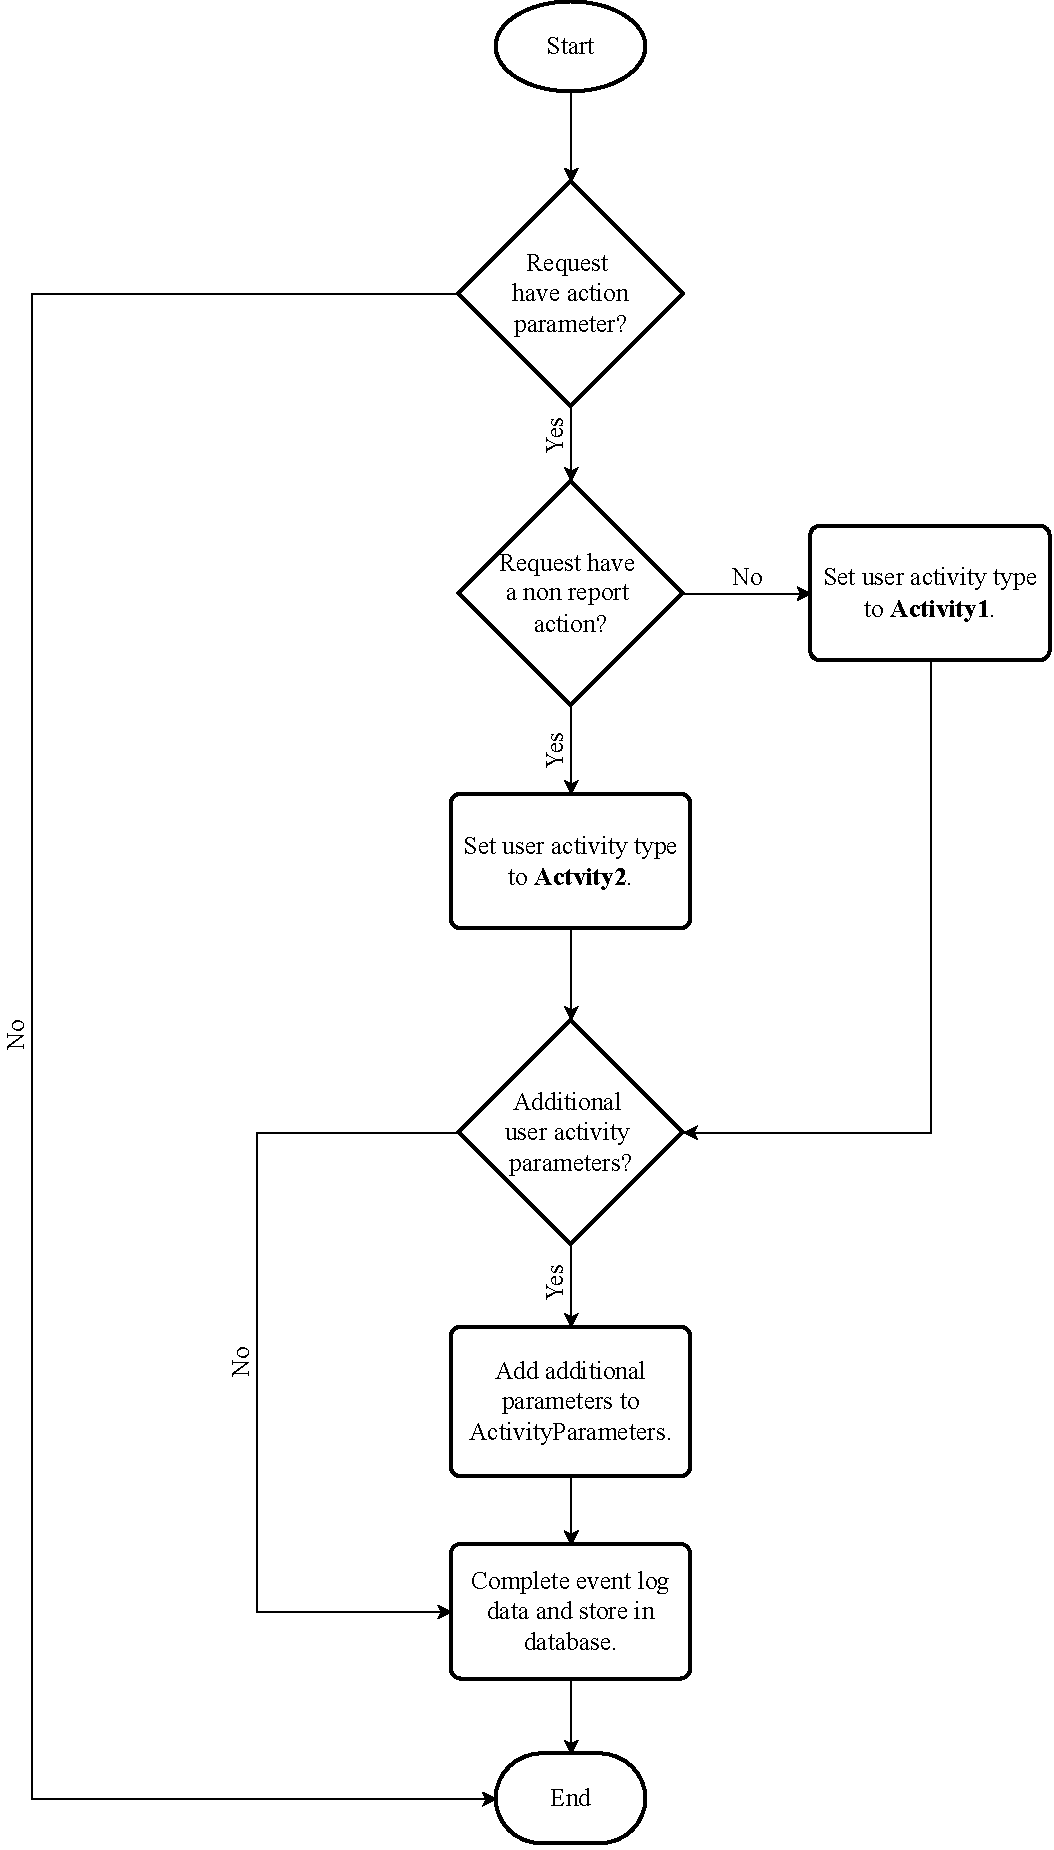
\includegraphics[width=0.8\textwidth]{Chapter2/DetailView_Flow/DetailView_Flow.pdf}
	\caption[Logging point operation for test system]
	{\textit{Logging point operation for test system}}\label{fig:ch3_loggingProcess}
\end{figure}

\clearpage

\subsubsection{Obtaining the element of user-based event}\label{sec:ch2_ElementObtaining}
In \Cref{sec:ch2_webApplicationArchitecture} the user-based activity event will be using a \textit{HTTP request} to send to the server when the user interacted with an \textit{HTML element}. For the functional requirements activity type (F/R 1.5.3) and metadata (F/R 1.5.6) in \Cref{tbl:ch2_keyLoggingAttributes} the \textit{HTML element} needs to be obtained to get the element's tag and identification text.\par This can be difficult to obtain due to \textit{bubbling}\footnote{\textbf{Bubbling} is when an event happens on an element, it first runs the handlers on it, then on its parent, then up on other ancestors. \cite{EventBubbling}.} that may occur when searching for the element that the user specifically interacted with. \Cref{fig:ch2_event_bubbling} is the event bubbling propagation.

\begin{figure}[!htb]
	\centering % cent the figure
	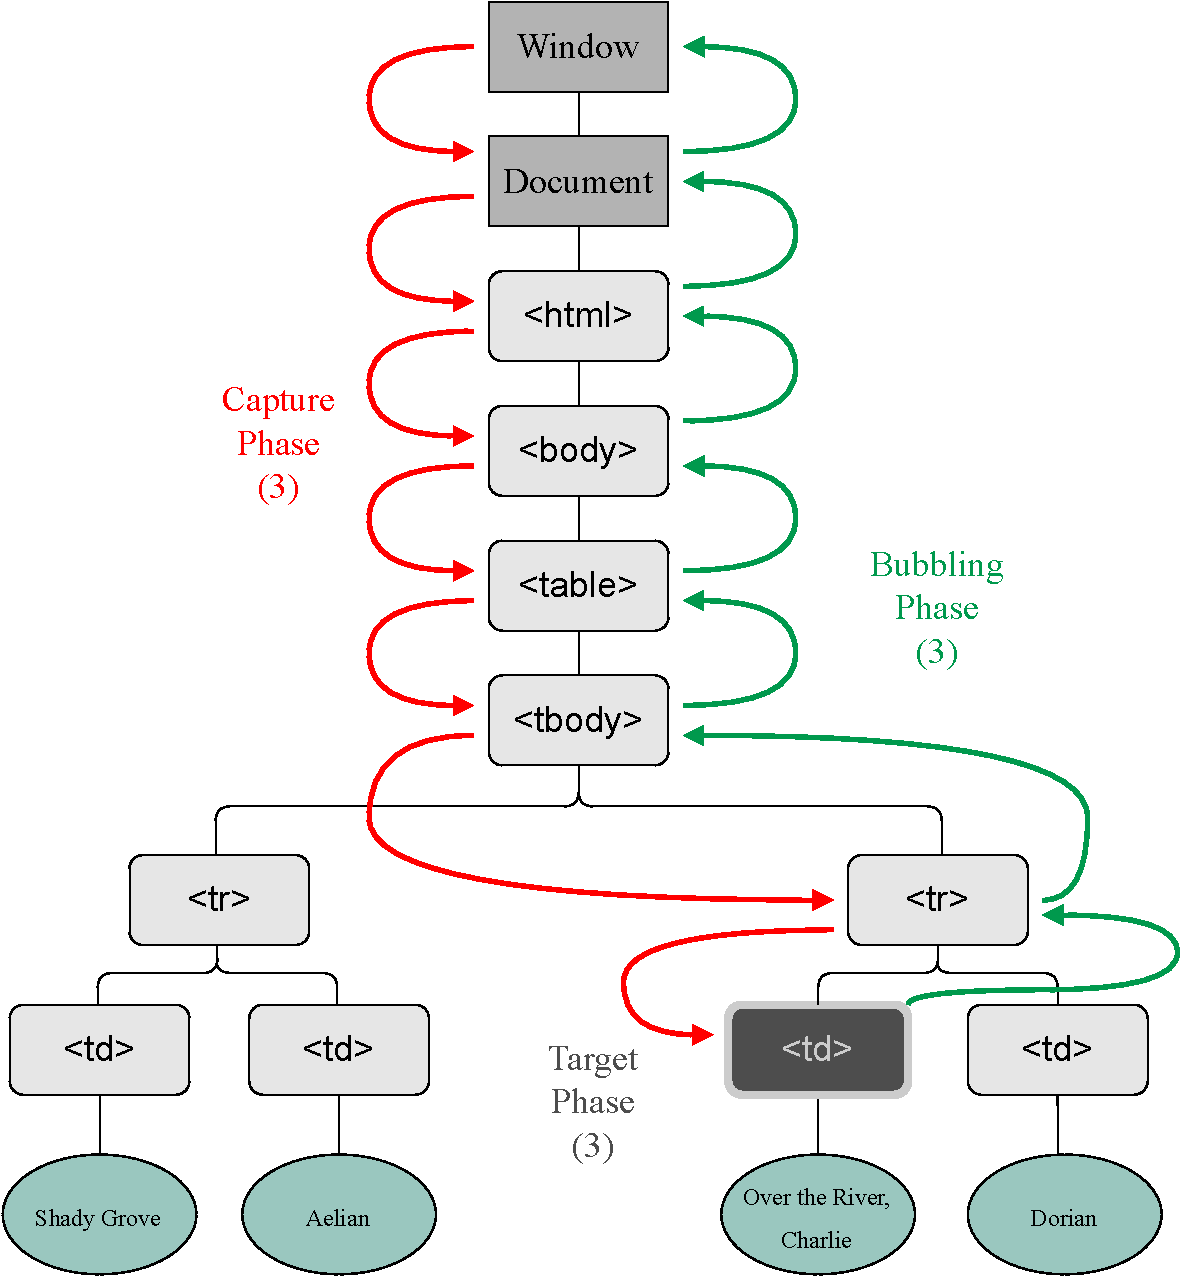
\includegraphics[width=0.8\textwidth]{Chapter2/event_bubbling/event_bubbling.pdf}
	\caption[JavaScript event propagation]
	{\textit{JavaScript event propagation~\cite{EventBubbling}}}\label{fig:ch2_event_bubbling}
\end{figure}

In \Cref{fig:ch2_event_bubbling} is the event propagation example of a child element that has been clicked on which executes a DOM event. The event propagation consists of three phases~\cite{EventBubbling}:

\begin{itemize}
	\item \textit{Capturing phase:} The event propagates downwards to the targeted element that the user interacted with.
	\item \textit{Target phase:} The event reaches the targeted element to execute the DOM event.
	\item \textit{Bubbling phase:} The event bubbles up from the targeted element
\end{itemize}

Capturing the targeted element may be difficult as some web pages may have more complex HTML, which can cause event propagation to fail to obtain the correct element information that the user interacted with. In such cases, it is more accurate to obtain the targeted element by identifying the last known element that the user hovered over on the user interface, as another DOM event may have started during the initial element's event.\par \Cref{fig:ch3_element_event_capturing} shows the flow diagram to capture the element that the user interacted with for the user-based activity log. This code segment will be initiated during the \texttt{beforeSend} operation of the \textit{AJAX request} to filter HTML elements by predefined allowed elements. Filtering the element tag names ensures that unwanted, more complex elements or basic elements that are not expected to be the initiator of the event, will be excluded. 

\begin{figure}[!htb]
	\centering % cent the figure
	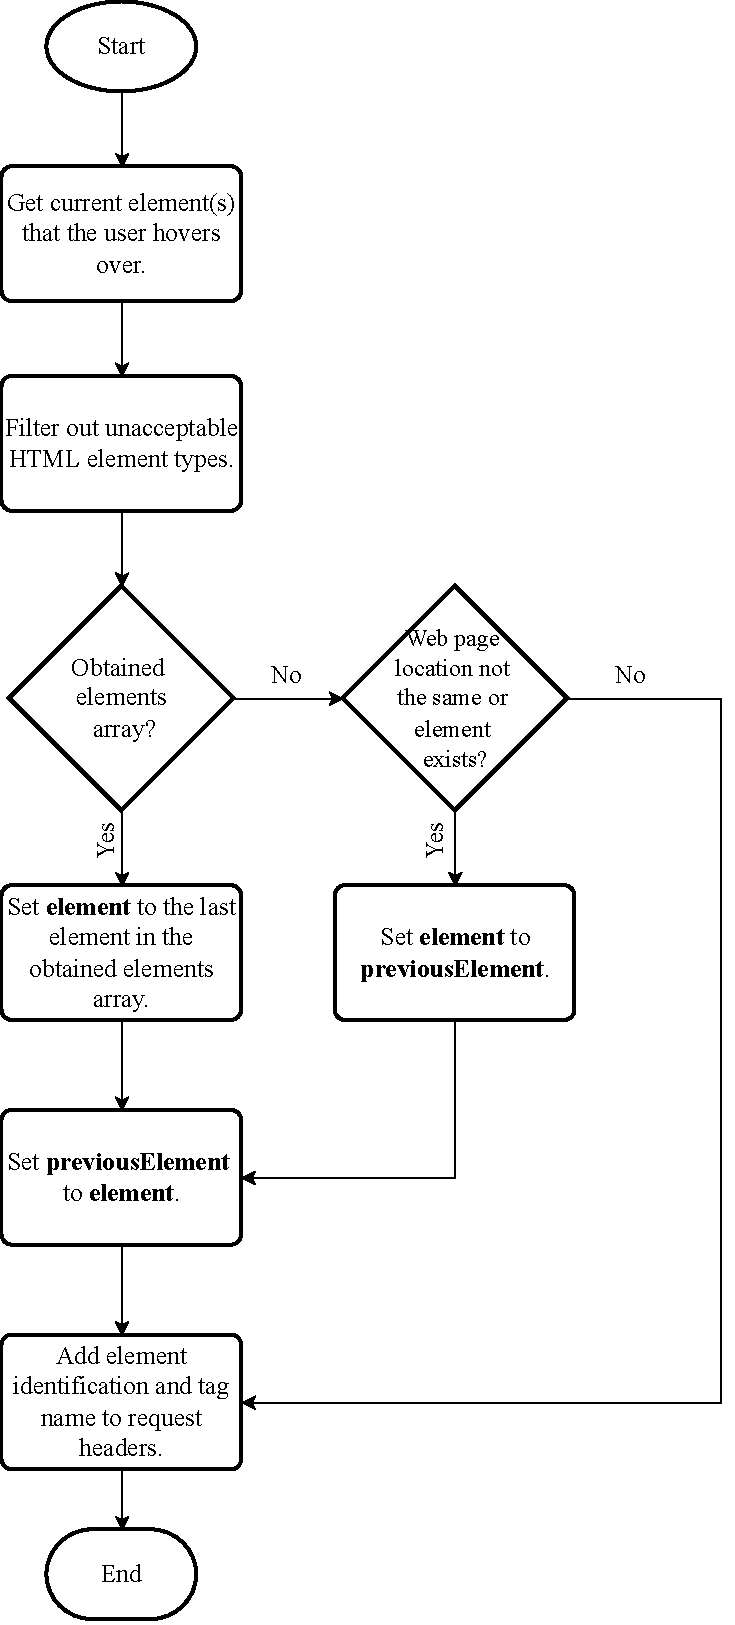
\includegraphics[width=0.55\textwidth]{Chapter2/element_capturing/element_capturing.pdf}
	\caption[HTML element capturing flow diagram]
	{\textit{HTML element capturing flow diagram}}\label{fig:ch3_element_event_capturing}
\end{figure}

If the web location has already changed or no element exists, the contents of the page may have already changed during the event propagation. Therefore, the last known element that the user hovered over must be used, as it is most likely to be the element that the user interacted with. This approach ensures that there is always an element that has been detected and parsed with the request header in most UI changes.

\clearpage

\subsection{Log analysis}\label{sec:ch3_implementationLogAnalysis}
In \Cref{ch2:sec_system_utilisation_analysis}, the functional requirements for log analysis are defined. For this implementation of log analysis, a custom log analysis tool is created to:

\begin{itemize}
\item Visually present user-based event logs through the log analysis tool as required in \Cref{tbl:ch2_logAnalysisToolFR}.
\item Filter user-based event logs through different criteria described in \Cref{tbl:ch2_utilisationCategories}.
\item Analyse logs for maintenance prioritisation as shown in \Cref{tbl:ch2_maintenancePriortising}.
\end{itemize}

\section{Verification}
The log analysis tool will be used to verify the implementation of the logging mechanism on the test system. This system is created in a \texttt{.NET Framework} software environment and uses a \texttt{MySQL} database to store the logging events.

\subsection{Log attributes}
The captured log attributes of \Cref{tbl:ch3_Log_Attributes} that are captured by the logging points are shown in \Cref{fig:ch3_UAT_menu}.

\begin{figure}[!htb]
	\centering % cent the figure
	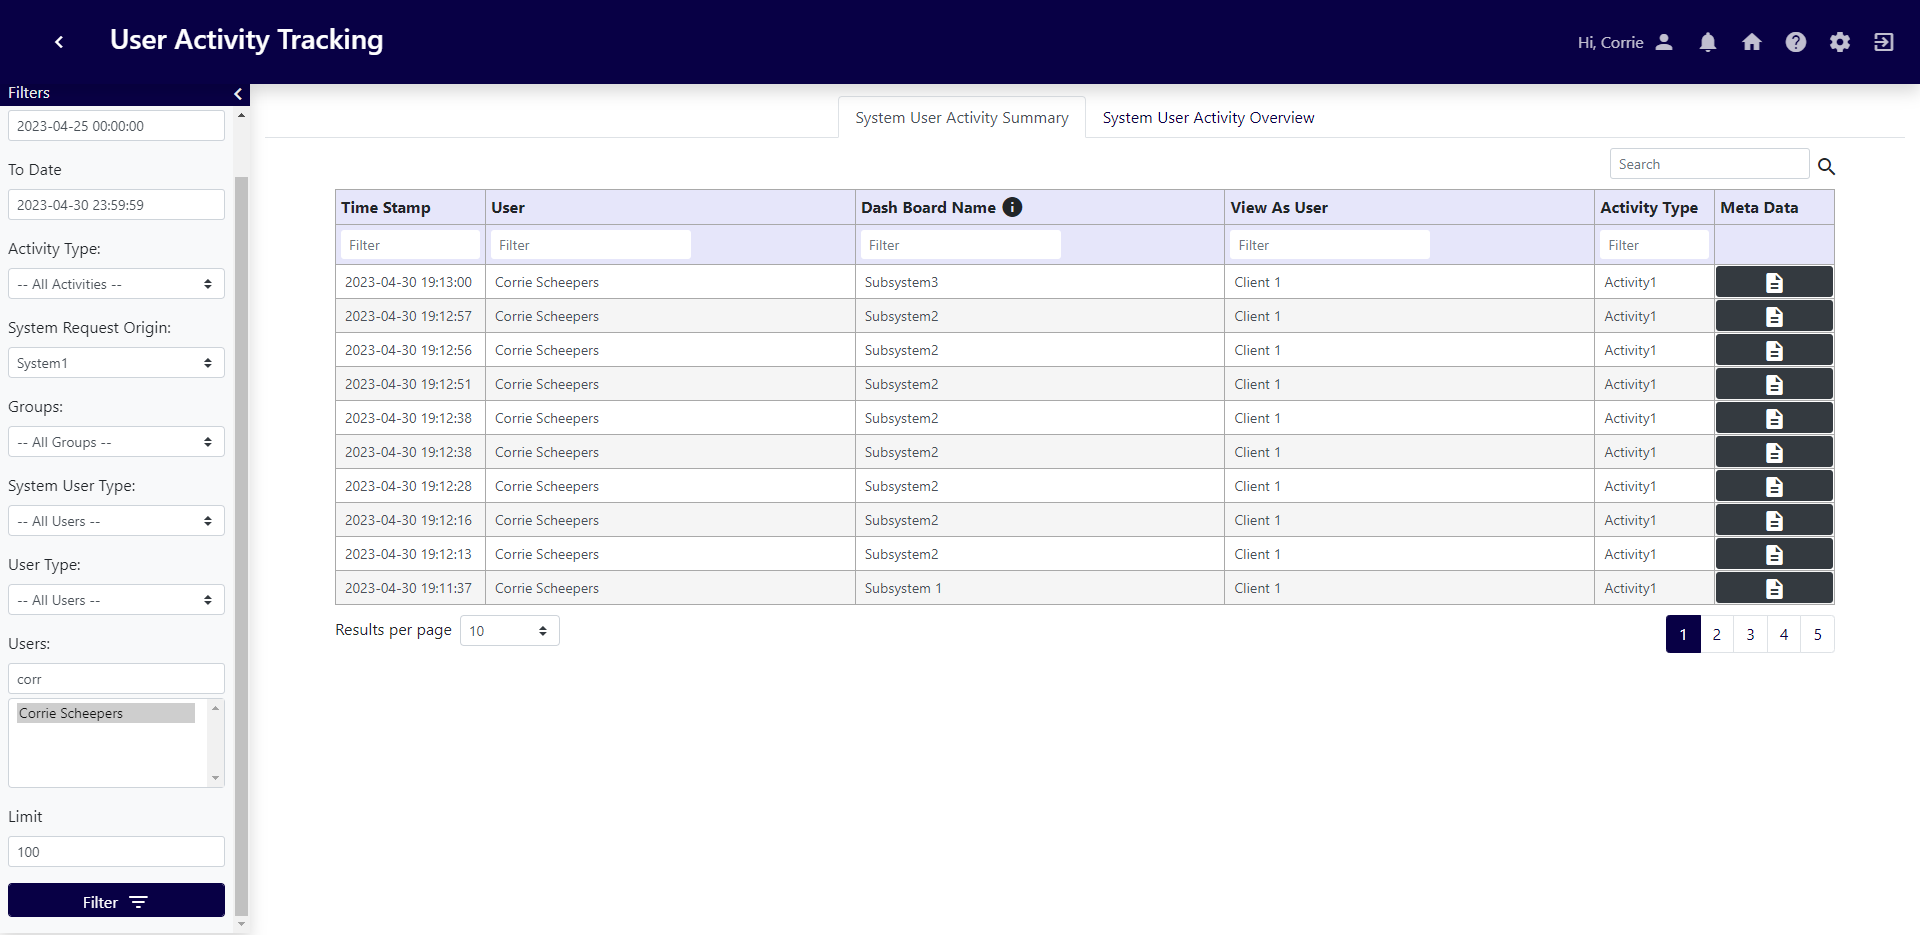
\includegraphics[width=0.99\linewidth]{img/ch3/analysis/UAT_menu.png}
	\caption[Interactive user activity viewer]
	{\textit{Interactive user activity viewer}}\label{fig:ch3_UAT_menu}
\end{figure}

\Cref{fig:ch3_UAT_menu} confirms that the required log attributes defined in \Cref{tbl:ch3_Log_Attributes} are being tracked for the test systems. The user interface created to display the logs is designed to be more understandable for users who analyze the logs. The meta-data is displayed in a \texttt{JSON} format as in \Cref{fig:ch3_JSON_Test_Result}.

\clearpage

\begin{figure}[!htb]
	\centering % cent the figure
	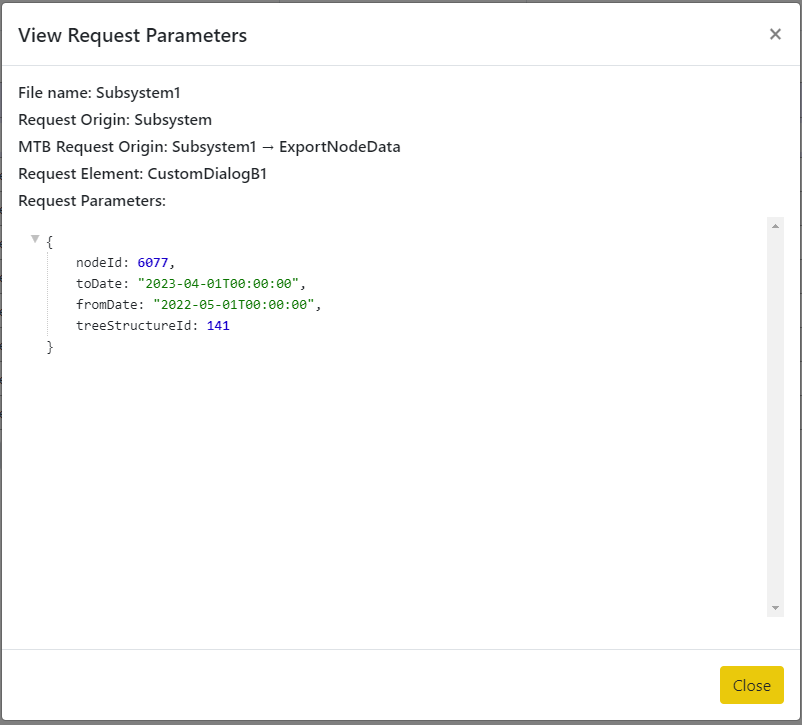
\includegraphics[width=0.65\linewidth]{img/ch3/analysis/UAT_request_params.png}
	\caption[JSON test request parameter data]
	{\textit{JSON test request parameter data}}\label{fig:ch3_JSON_Test_Result}
\end{figure}

\Cref{fig:ch3_JSON_Test_Result} includes additional parameters described in \Cref{fig:ch3_MetadataJson}. The \texttt{RequestElementID} is obtained using the element capturing method described in \Cref{fig:ch3_element_event_capturing}, while the other metadata parameters are captured using the built-in methods available in \texttt{C\#}.

\subsection{Log analysis}
The log analysis of the obtained logs shown in \Cref{fig:ch3_UAT_menu} is done in the same interactive dashboard. \Cref{fig:ch3_UAT_menuAnalysis} is a comparison of the obtained logs for the subsystems.

\begin{figure}[!htb]
	\centering % cent the figure
	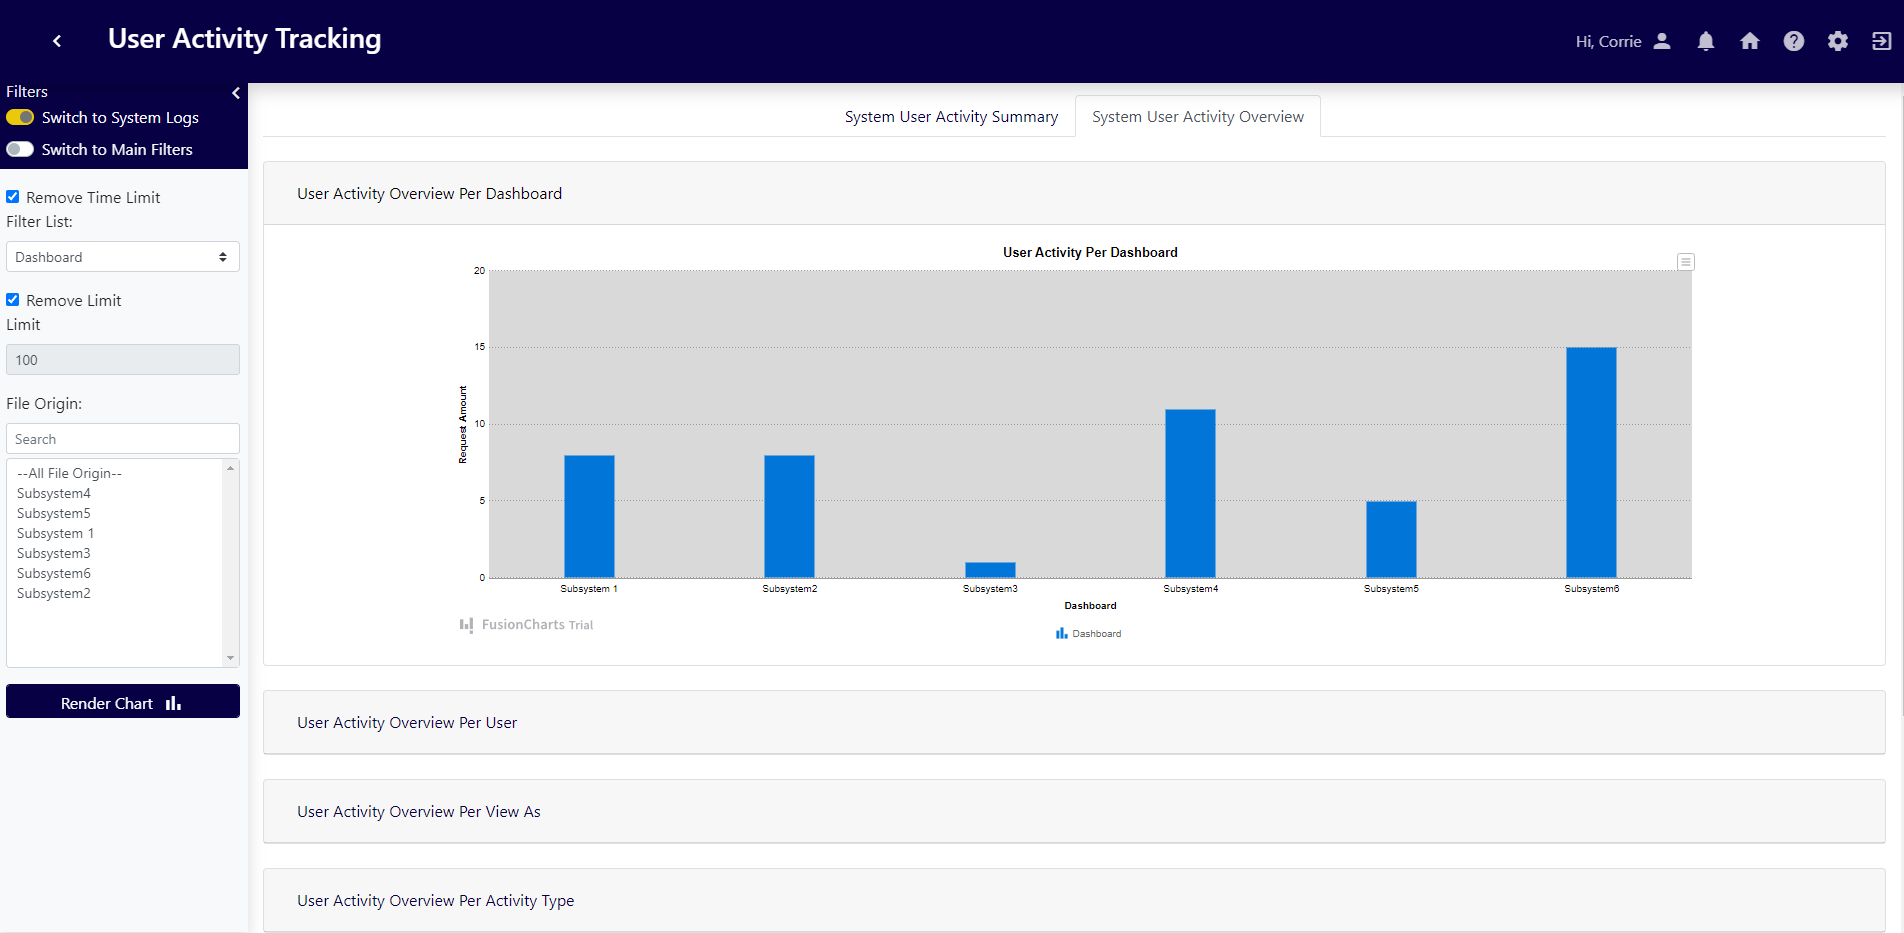
\includegraphics[width=0.99\linewidth]{img/ch3/analysis/UAT_menu_analysis.png}
	\caption[Interactive user activity viewer]
	{\textit{Interactive user activity viewer}}\label{fig:ch3_UAT_menuAnalysis}
\end{figure}

\clearpage

\Cref{tbl:ch2_utilisationCategories} provides the functional requirements for various utilization categories. By comparing these categories to each other in the obtained user logs, different categories can be compared, as shown in \Cref{fig:ch3_UAT_menuAnalysis}. Furthermore, \Cref{fig:ch3_UAT_menuActivities} compares different types of user activities.

\begin{figure}[!htb]
	\centering % cent the figure
	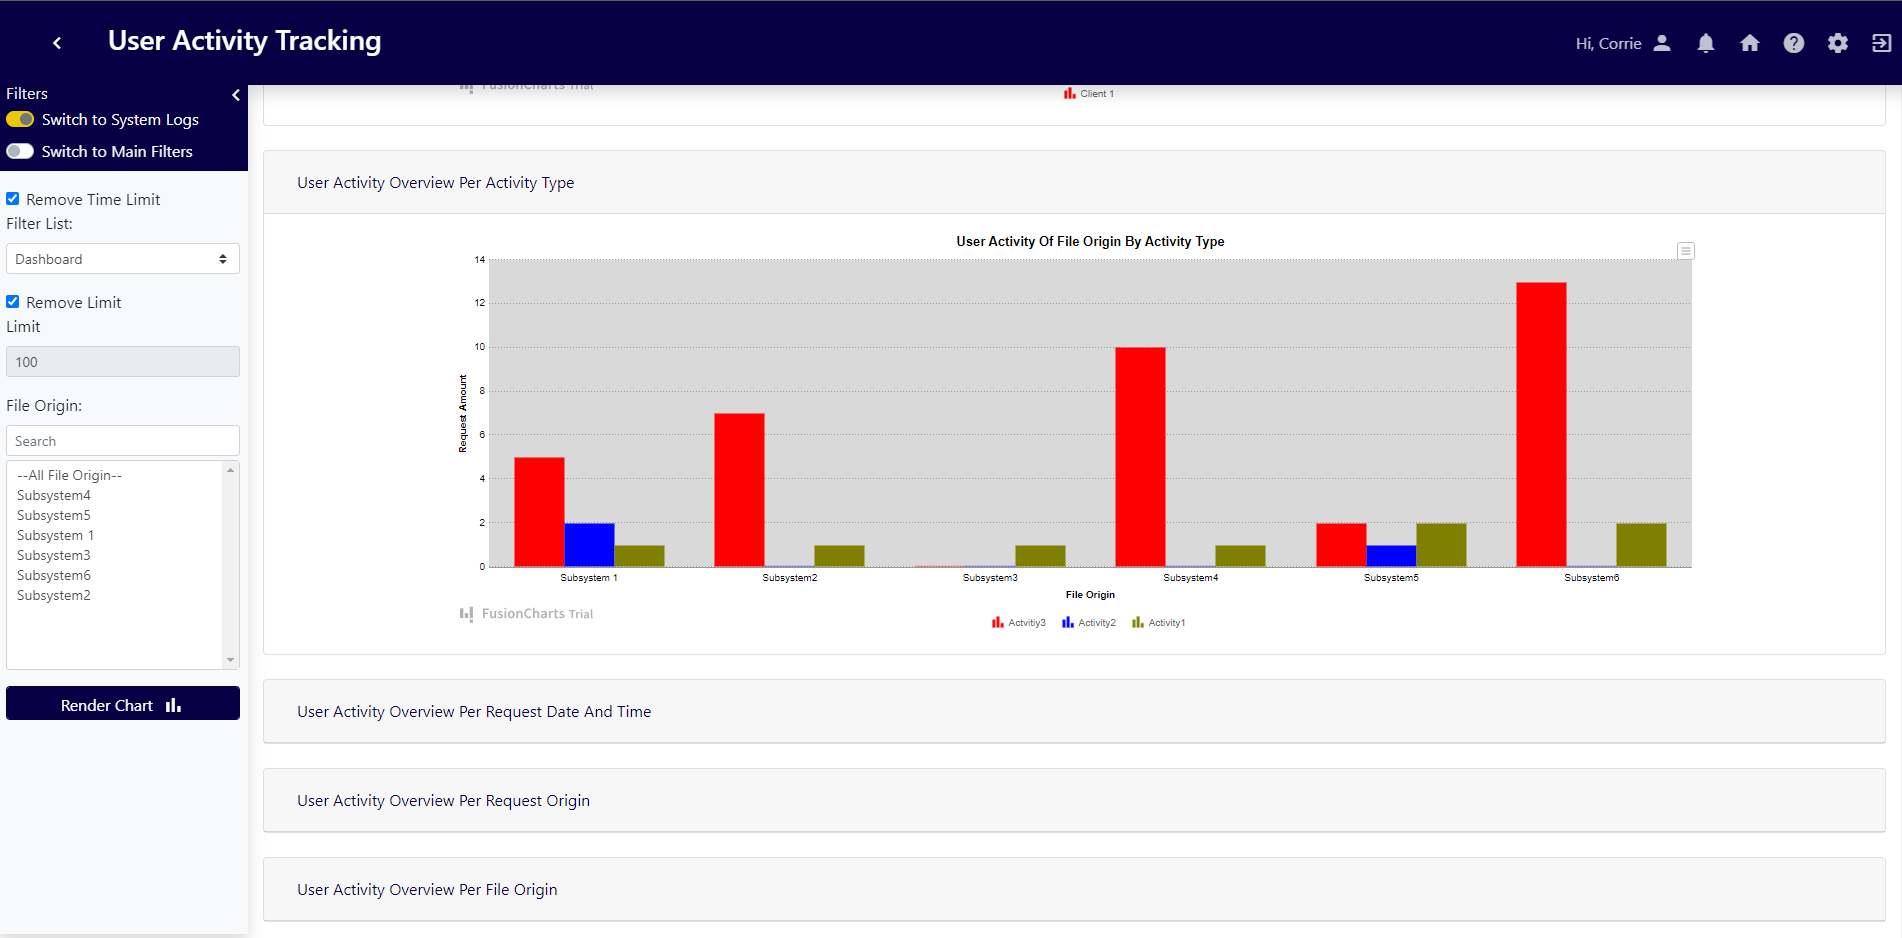
\includegraphics[width=0.99\linewidth]{img/ch3/analysis/UAT_menu_activities.png}
	\caption[Interactive user activity log analysis]
	{\textit{Interactive user activity log analysis}}\label{fig:ch3_UAT_menuActivities}
\end{figure}

\subsection{Maintenance priortising}
For the test system, maintenance prioritisation recommendations can be made as described in \Cref{sec:ch2_utilisationImprovements}. A rating system can be used to rank the most critical software systems that need to be prioritised, which can aid in software maintenance efforts.\par Using \Cref{eq:ch2_maintenanceFactorSimplified} the maintenance priority factor $M_{PF}$ can be determined for a set of systems {$S1,~S_2,~...,~S_N$} which has captured user activities per system $A_X$. The system will also have several users linked to each system $P_X$. These parameters are set for the test system as in \Cref{tbl:ch3_testData}.

\begin{table}[!htb]
	\centering
	\caption[Data for validating test system]
	{\textit{Data for validating test system}}
	\label{tbl:ch3_testData}
	\begin{tabularx}{\textwidth}{|X|X|X|}
		\hline \textbf{System ($S_X$)} & \textbf{Users per system ($P_X$)} & \textbf{Number of events ($A_X$)} \\
		\hline $S_1$ & 226 & 11 \\
		\hline $S_2$ & 269 & 5 \\
		\hline $S_3$ & 156 & 8 \\
		\hline $S_4$ & 155 & 1 \\
		\hline $S_5$ & 145 & 13 \\
		\hline $S_6$ & 154 & 8 \\
		\hline
	\end{tabularx}
\end{table}

The activities in \Cref{tbl:ch3_testData} were generated by a single user who navigated through and interacted with the system, as shown in \Cref{fig:ch3_UAT_menuActivities,fig:ch3_UAT_menuAnalysis}. To compare the effect of the total number of user activities per system, we focus on $S_3$ to $S_6$, which have similar numbers of active users who can access the system. For the test system $S$, it is expected that $S_1$ will have the highest maintenance priority factor, given that it has:

\begin{itemize}
	\item The second highest number of users linked to it. This should increase its normalised active user factor.
	\item It has the second-highest number of observed user events that were captured.
\end{itemize}

$S_4$ has the least total number of user events but has about the same number of users linked to it. This should have the lowest maintenance factor as a lower number of activities will indicate that the system is not used as much as systems like $S_3$ and $S_6$. These other two systems have higher captured user events.\par Using \Cref{eq:ch2_priorityNormalised} to calculate each subsystem's normalised priority factor using the number of users that have access to the system; also using \Cref{eq:ch2_eventNormalised} to calculate the normalised activities, the results are shown in \Cref{tbl:apx_testB_Normilised}.


    \begin{xltabular}{\textwidth}{|X|X|X|X|X|X|X|}
        \caption[Test data]
        {\textit{Test data}}
        \label{tbl:apx_testB_Normilised} \\
        
        \hline
        \textbf{$S_{X}$} & \textbf{$P_X$} & \textbf{$P_N$}  & \textbf{$A_X$} & \textbf{$A_N$} & \textbf{$M_{PF}$} & \textbf{$P_{R}$} \\
        \hline
        \endfirsthead

        \multicolumn{7}{c}
        {\tablename\ \thetable{} -- continued from previous page} \\
        \hline
        \textbf{$S_{X}$} & \textbf{$P_X$} & \textbf{$P_N$}  & \textbf{$A_X$} & \textbf{$A_N$} & \textbf{$M_{PF}$} & \textbf{$P_{R}$} \\ 
        \endhead

        \multicolumn{7}{|r|}{{Continued on next page}} \\ \hline
        \endfoot

        \hline
        \endlastfoot
    $S_1$ & 226 & 0.6504 & 11 & 0.8333 & 0.5420 & 1 \\ \hline
 $S_2$ & 269 & 1.0000 & 5 & 0.3333 & 0.3333 & 2 \\ \hline
 $S_3$ & 156 & 0.0813 & 8 & 0.5833 & 0.0474 & 3 \\ \hline
 $S_6$ & 154 & 0.0650 & 8 & 0.5833 & 0.0379 & 4 \\ \hline
 $S_4$ & 155 & 0.0732 & 1 & 0.0000 & 0.0000 & 5 \\ \hline
 $S_5$ & 146 & 0.0000 & 13 & 1.0000 & 0.0000 & 5 \\ \hline
    \end{xltabular}
    

In \Cref{tbl:apx_testB_Normilised}, $P_N$ for $S_1$ and $S_2$ is the highest, as most users have access to them. Additionally, $S_1$ and $S_5$ have the highest $A_N$ rating, indicating that they were the most used systems. As previously stated, it is expected that $S_1$ will require the most maintenance activities. The systems with lower maintenance activities and still have similar active users linked to them have a lower maintenance priority factor.

\clearpage

\section{Case studies}

\subsection{Case study identification}
To fully examine the application of this study, three separate case studies will be used. All the case studies are web-based applications where users need credentials to log in and have restricted access to some parts of the system. These case studies are identified in \Cref{tbl:ch3_caseStudies}.

\begin{table}[!htb]
	\centering
	\caption[Case studies]
	{\textit{Case studies}}
	\label{tbl:ch3_caseStudies}
	\begin{tabularx}{\textwidth}{|X|X|X|}
		\hline \textbf{Case study} & \textbf{Software framework} & \textbf{Description} \\
		\hline System A & \texttt{ASP.NET Core Web SDK} & \RaggedRight Energy management software system that consists of both internal and external client users. \\
		\hline System B & \texttt{PHP} & \RaggedRight An older energy management software system that consists of both internal and external client users. \\
		\hline System C & \texttt{ASP.NET Core Web SDK} & \RaggedRight Administrative software system used by internal users of a company. Consist mostly of configuration tools for System A and System B and is only accessible to internal users. \\
		\hline
	\end{tabularx}
\end{table}

These case studies in \Cref{tbl:ch3_caseStudies} are being used because they have different use cases and software framework implementations. System A and System B are similar software systems but use older and newer software frameworks. Due to these differences, the logging mechanism needs to be implemented in different ways to capture user-based activities.\par For the three subsystems, the following results will be obtained:

\begin{itemize}
\item Defining the most important user activity types.
\item Defining how the logging point is implemented for the specific subsystem to obtain the user-based event logs.
\item Only the subsystems' user activities that are in the upper quartile is used for each case study that was recorded in October 2022.
\item The normalised priority for each subsystem of the main system will be calculated using \Cref{eq:ch2_priorityNormalised} based on the active users who have access to the system.
\item The normalised activities of each subsystem will be calculated using \Cref{eq:ch2_eventNormalised}.
\item The maintenance priority factor will be calculated for each of the subsystems using \Cref{eq:ch2_maintenanceFactorSimplified}.
\item The normalisation of the priority factor is only for users who have access to the subsystem and interacted with the subsystem. All other users who do not meet this requirement will be excluded.
\end{itemize}

\subsection{Case study A results}
System A is a \texttt{ASP.NET Core Web SDK} software system. The software system has 3 basic user activity types as shown in \Cref{tbl:ch3_systemAActivityTypes}.

\begin{table}[!htb]
	\centering
	\caption[System A activity types]{\textit{System A activity types}}
	\label{tbl:ch3_systemAActivityTypes}
	\begin{tabularx}{\textwidth}{|X|l|X|}
		\hline \textbf{Activity} & \textbf{Functional requirement} & \textbf{Description} \\
		\hline \texttt{Dash} & \ref{fr:uatType1} & \RaggedRight This activity type detects when a user has navigated to a certain subsystem. \\ 
		\hline \texttt{DetailView} & \ref{fr:uatType3} & \RaggedRight This general activity type is for all other activities that the user initiates that send \textit{HTTP request} back to the server.  \\
		\hline \texttt{Report} & \ref{fr:uatType3} & \RaggedRight The other main function of the system is for reporting purposes. \\ 
		\hline
	\end{tabularx}
\end{table}

To capture the user activity types defined in \Cref{tbl:ch3_systemAActivityTypes}, the logging point is placed in a central place in the software code. Using action filters that are available in \texttt{ASP.NET Core}, the single logging point can be placed in the software system to capture the user-based event logs.\par Additional metadata, such as the HTML element associated with the user-based event, is also captured. Using the HTML event capturing method shown in \Cref{fig:ch3_element_event_capturing}, the element information is captured and stored along with the request parameters in the same format as in \Cref{fig:ch3_MetadataJson}. \Cref{fig:ch3_caseABreakdown} is the total captured user activities breakdown of the user activity types of \Cref{tbl:ch3_systemAActivityTypes}.

\begin{figure}[!htb]
	\centering % cent the figure
	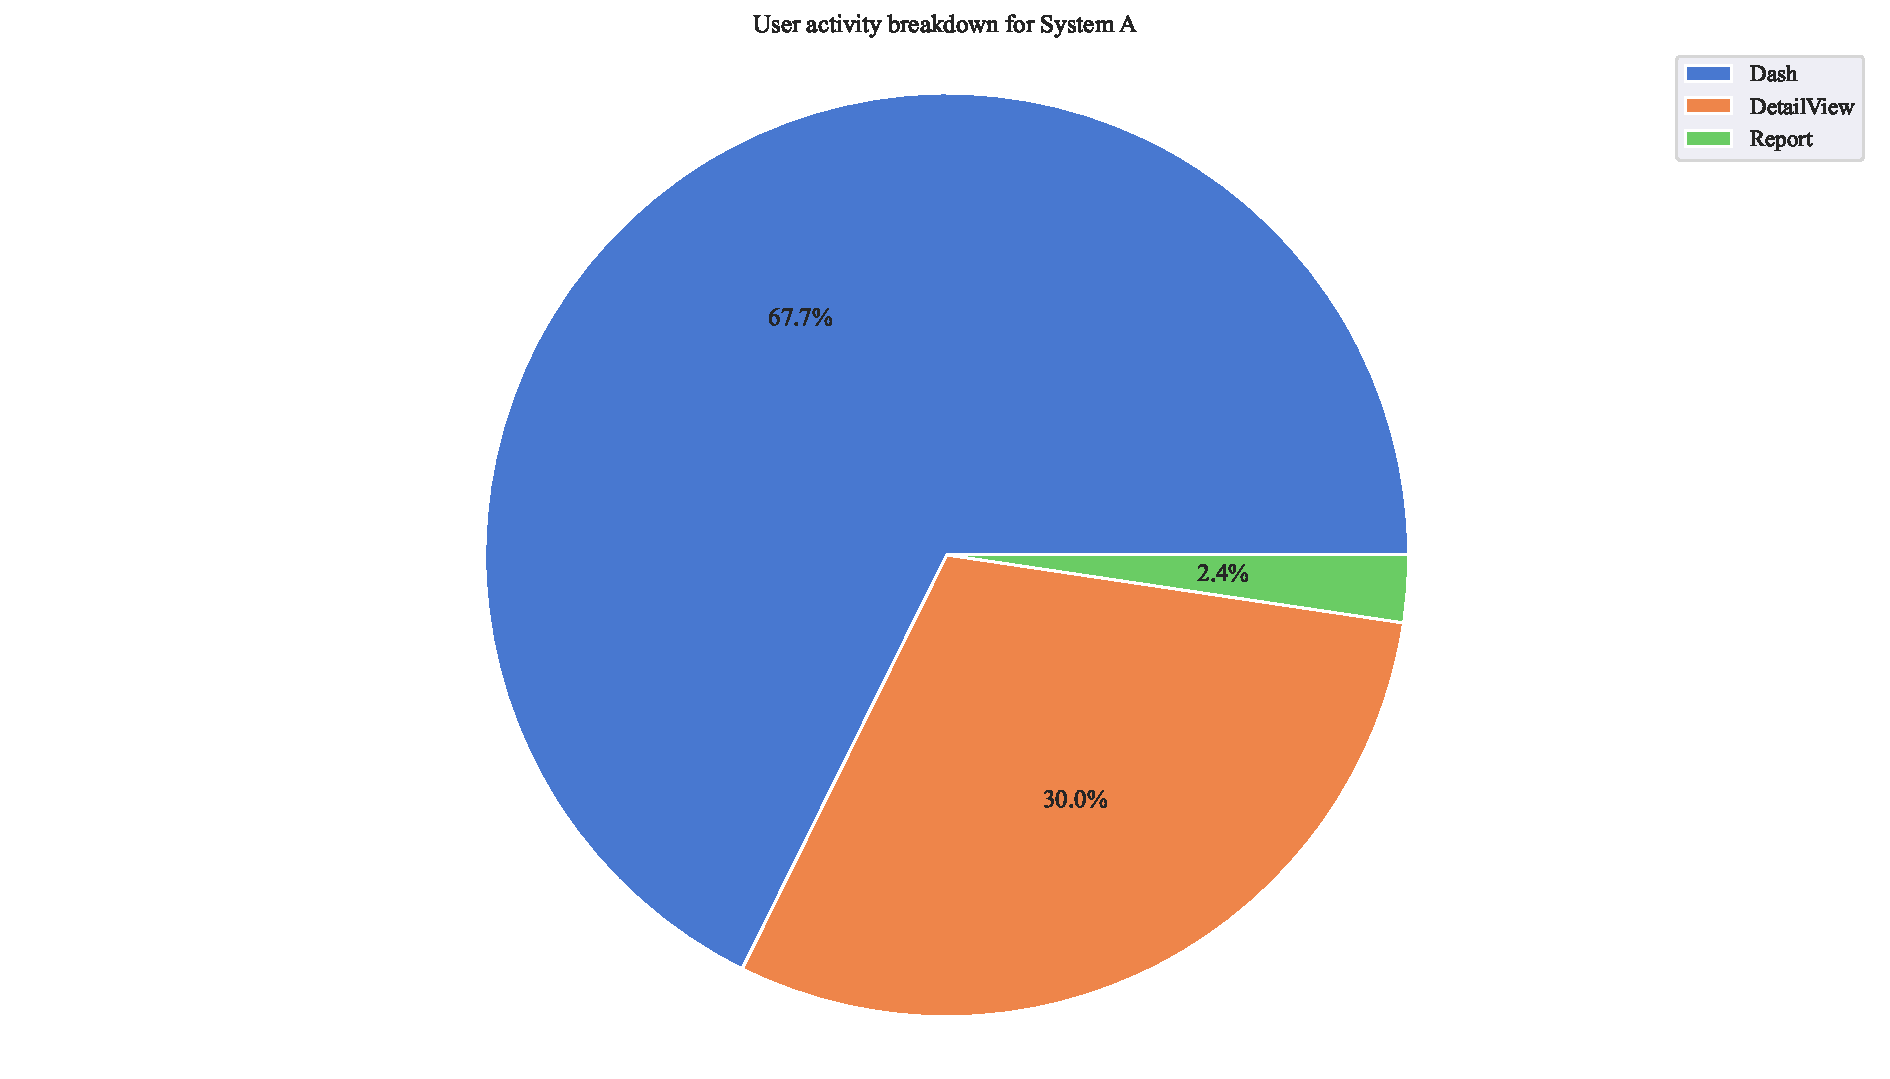
\includegraphics[width=0.95\linewidth]{img/ch3/analysis/case_A_breakdown.pdf}
	\caption[User activity types breakdown of System A]
	{\textit{User activity types breakdown of System A}}\label{fig:ch3_caseABreakdown}
\end{figure} 

\clearpage

The \Cref{fig:ch3_caseABreakdown} the majority of the user activities for the case study A's subsystems is the Dash user activity type. Most of the subsystems don't have many inputs for the user to enter data on the system. It provides information back to the user that causes the majority of the user activities. 

\subsubsection{Maintenance prioritisation}
The maintenance prioritisation factor for the upper quartile user activities of the subsystem for case study A is calculated in \Cref{tbl:apx_caseA}.


    \begin{xltabular}{\textwidth}{XPPPP}
        \caption[Case study A's upper quartile maintenance pefromance]
        {\textit{Case study A's upper quartile maintenance pefromance}}
        \label{tbl:apx_caseA} \\
        \toprule
         \thead{$S_{X}$} & \thead{$P_N$}  & \thead{$A_N$} & \thead{$M_{PF}$} & \thead{$P_{R}$} \\
        \midrule
        \endfirsthead

        \caption[]{\continueCaption} \\
        \toprule
        \thead{$S_{X}$} & \thead{$P_N$}  & \thead{$A_N$} & \thead{$M_{PF}$} & \thead{$P_{R}$} \\
        \midrule
        \endhead

        \midrule
        \multicolumn{5}{r}{\continueText} \\ 
        \endfoot
        \endlastfoot
    \rowcolor{lightgray} $S_{538}$ & 1.0000 & 0.5281 & 0.5281 & 1 \\ 
  $S_{413}$ & 0.5469 & 0.8423 & 0.4606 & 2 \\ 
 \rowcolor{lightgray} $S_{570}$ & 0.4531 & 0.9041 & 0.4097 & 3 \\ 
  $S_{582}$ & 0.2531 & 1.0000 & 0.2531 & 4 \\ 
 \rowcolor{lightgray} $S_{412}$ & 0.8344 & 0.2753 & 0.2297 & 5 \\ 
  $S_{546}$ & 0.6281 & 0.2240 & 0.1407 & 6 \\ 
 \rowcolor{lightgray} $S_{580}$ & 0.2250 & 0.5923 & 0.1333 & 7 \\ 
  $S_{454}$ & 0.4781 & 0.2392 & 0.1144 & 8 \\ 
 \rowcolor{lightgray} $S_{577}$ & 0.2656 & 0.3755 & 0.0997 & 9 \\ 
  $S_{593}$ & 0.2031 & 0.4496 & 0.0913 & 10 \\ 
 \rowcolor{lightgray} $S_{568}$ & 0.4719 & 0.1315 & 0.0621 & 11 \\ 
  $S_{445}$ & 0.4813 & 0.1166 & 0.0561 & 12 \\ 
 \rowcolor{lightgray} $S_{735}$ & 0.2625 & 0.1487 & 0.0390 & 13 \\ 
  $S_{476}$ & 0.2844 & 0.0956 & 0.0272 & 14 \\ 
 \rowcolor{lightgray} $S_{729}$ & 0.2594 & 0.0976 & 0.0253 & 15 \\ 
  $S_{404}$ & 0.7000 & 0.0338 & 0.0237 & 16 \\ 
 \rowcolor{lightgray} $S_{441}$ & 0.5563 & 0.0411 & 0.0229 & 17 \\ 
  $S_{600}$ & 0.2375 & 0.0808 & 0.0192 & 18 \\ 
 \rowcolor{lightgray} $S_{458}$ & 0.4500 & 0.0421 & 0.0189 & 19 \\ 
  $S_{469}$ & 0.4656 & 0.0358 & 0.0167 & 20 \\ 
 \rowcolor{lightgray} $S_{435}$ & 0.5156 & 0.0192 & 0.0099 & 21 \\ 
  $S_{581}$ & 0.4750 & 0.0200 & 0.0095 & 22 \\ 
 \rowcolor{lightgray} $S_{755}$ & 0.2812 & 0.0232 & 0.0065 & 23 \\ 
  $S_{753}$ & 0.2375 & 0.0258 & 0.0061 & 24 \\ 
 \rowcolor{lightgray} $S_{616}$ & 0.3219 & 0.0164 & 0.0053 & 25 \\ 
  $S_{503}$ & 0.4500 & 0.0099 & 0.0045 & 26 \\ 
 \rowcolor{lightgray} $S_{756}$ & 0.2375 & 0.0099 & 0.0024 & 27 \\ 
  $S_{428}$ & 0.2594 & 0.0071 & 0.0018 & 28 \\
        \bottomrule
    \end{xltabular}
    

\Cref{tbl:apx_caseA} shows the results of implementing \Cref{eq:ch2_priorityNormalised,eq:ch2_eventNormalised,eq:ch2_maintenanceFactorSimplified} to calculate the normalised priority ($P_N$), normalised activity ($A_X$), and maintenance factor ($M_{PF}$). The \Cref{tbl:apx_caseA} only contains the upper quartile subsystems of all the total subsystems of \Cref{tbl:apx_projectA_Normilised}. The results are visually presented in \Cref{fig:ch3_caseAAnalysis} collected from \Cref{tbl:apx_caseA} with the user activity breakdown.

\clearpage

\begin{figure}[!htb]
	\centering % cent the figure
	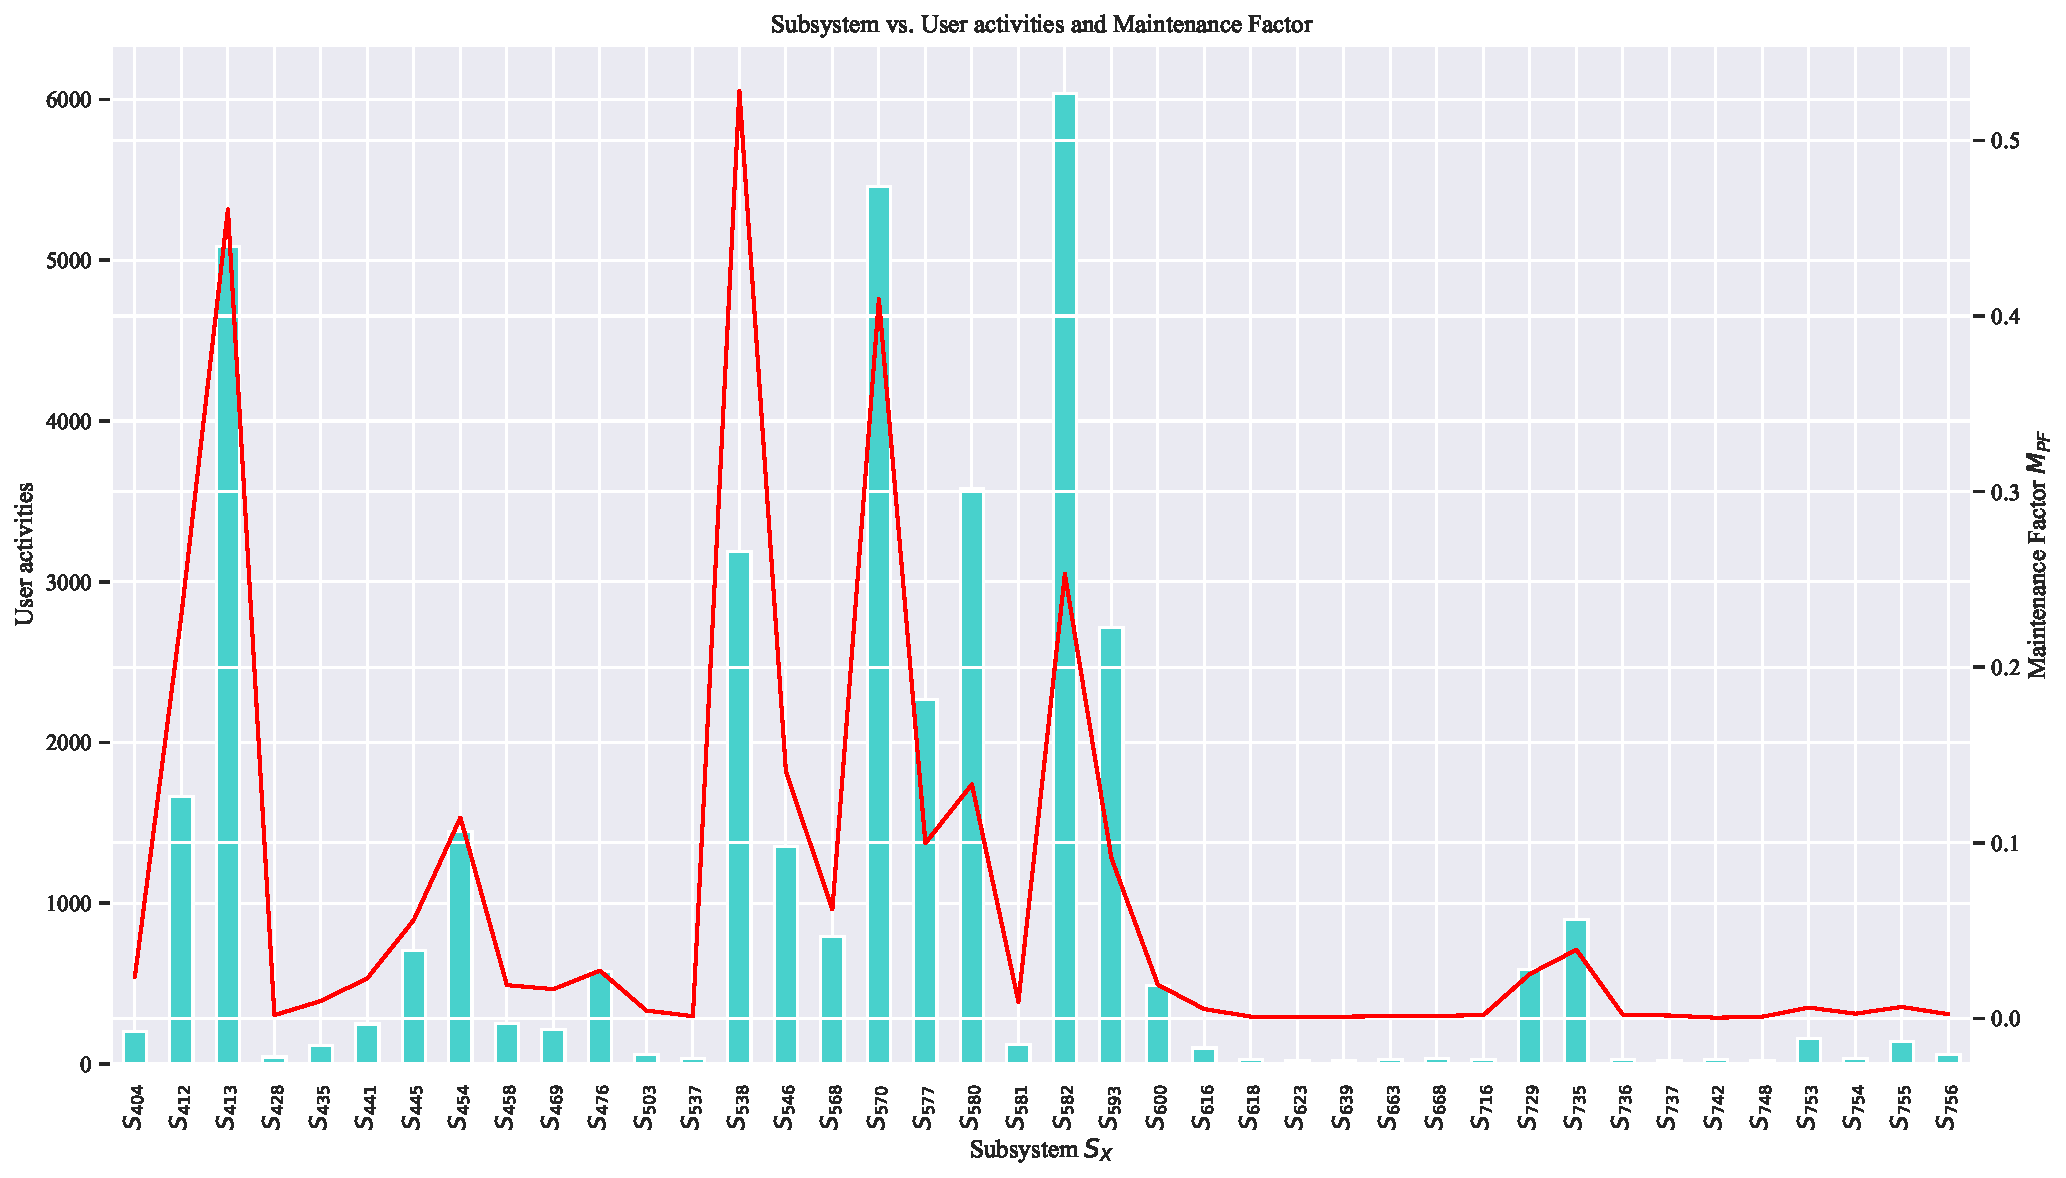
\includegraphics[width=0.95\linewidth]{img/ch3/analysis/case_A_subsystems_1.pdf}
	\caption[Maintenance performance calculation for system A]
	{\textit{Maintenance performance calculation for system A}}\label{fig:ch3_caseAAnalysis}
\end{figure}

\par In \Cref{fig:ch3_caseAAnalysis}, subsystem $S_{582}$ had the most user-based events generated, with an average of $72.75$ user-based events per user. The lower $P_N$ reduced its maintenance priority factor to be the $4_{th}$ highest for all subsystems. Subsystem $S_{538}$ had the $5^{th}$ highest number of recorded user-based activities and the most users that have access to the subsystem. The higher $P_N$ had a bigger impact on its maintenance performance factor.\par For systems such as $S_{413}$ the majority of the user activities were from actions that the user performed other than accessing the subsystem which is the DetailView user activity type. This is different from the other top five systems that had a majority of Dash user activity types. Users only viewed the content of the web page for that subsystem. From these results, the maintenance prioritisation should be for the systems in the order of $P_R$ in \Cref{tbl:apx_caseA}. 

\subsection{Case study B results}
System B is an older system than A and C that is primarily created in \texttt{PHP}. This system has the same type of user activities as System A's \Cref{tbl:ch3_systemAActivityTypes}. To capture the user types of \Cref{tbl:ch3_systemAActivityTypes} this system used multiple logging points.\par The use of the multiple logging points was to:

\begin{itemize}
	\item Ensure each subsystem's user activities could be captured as there wasn't any central point in the software architecture to capture the request. 
	\item The system consisted of groups of smaller software systems where the logging points could be added.
	\item Some adjustments had to be made to the logging points to ensure that the log's quality is maintained when it is captured. 
	\item Consistency was also important so each logging has some minor differences added to ensure that it can consistently capture certain user-based events. \
\end{itemize}

The logging points don't track any of the elements that the user interacted with the system. Only some of the request parameters are tracked for any of the user-based activities. The metadata will only contain the \texttt{RequestParameters} used in \Cref{fig:ch3_MetadataJson}. The user activity type breakdown for this case study is shown in \Cref{fig:ch3_caseBBreakdown}.

\begin{figure}[!htb]
	\centering % cent the figure
	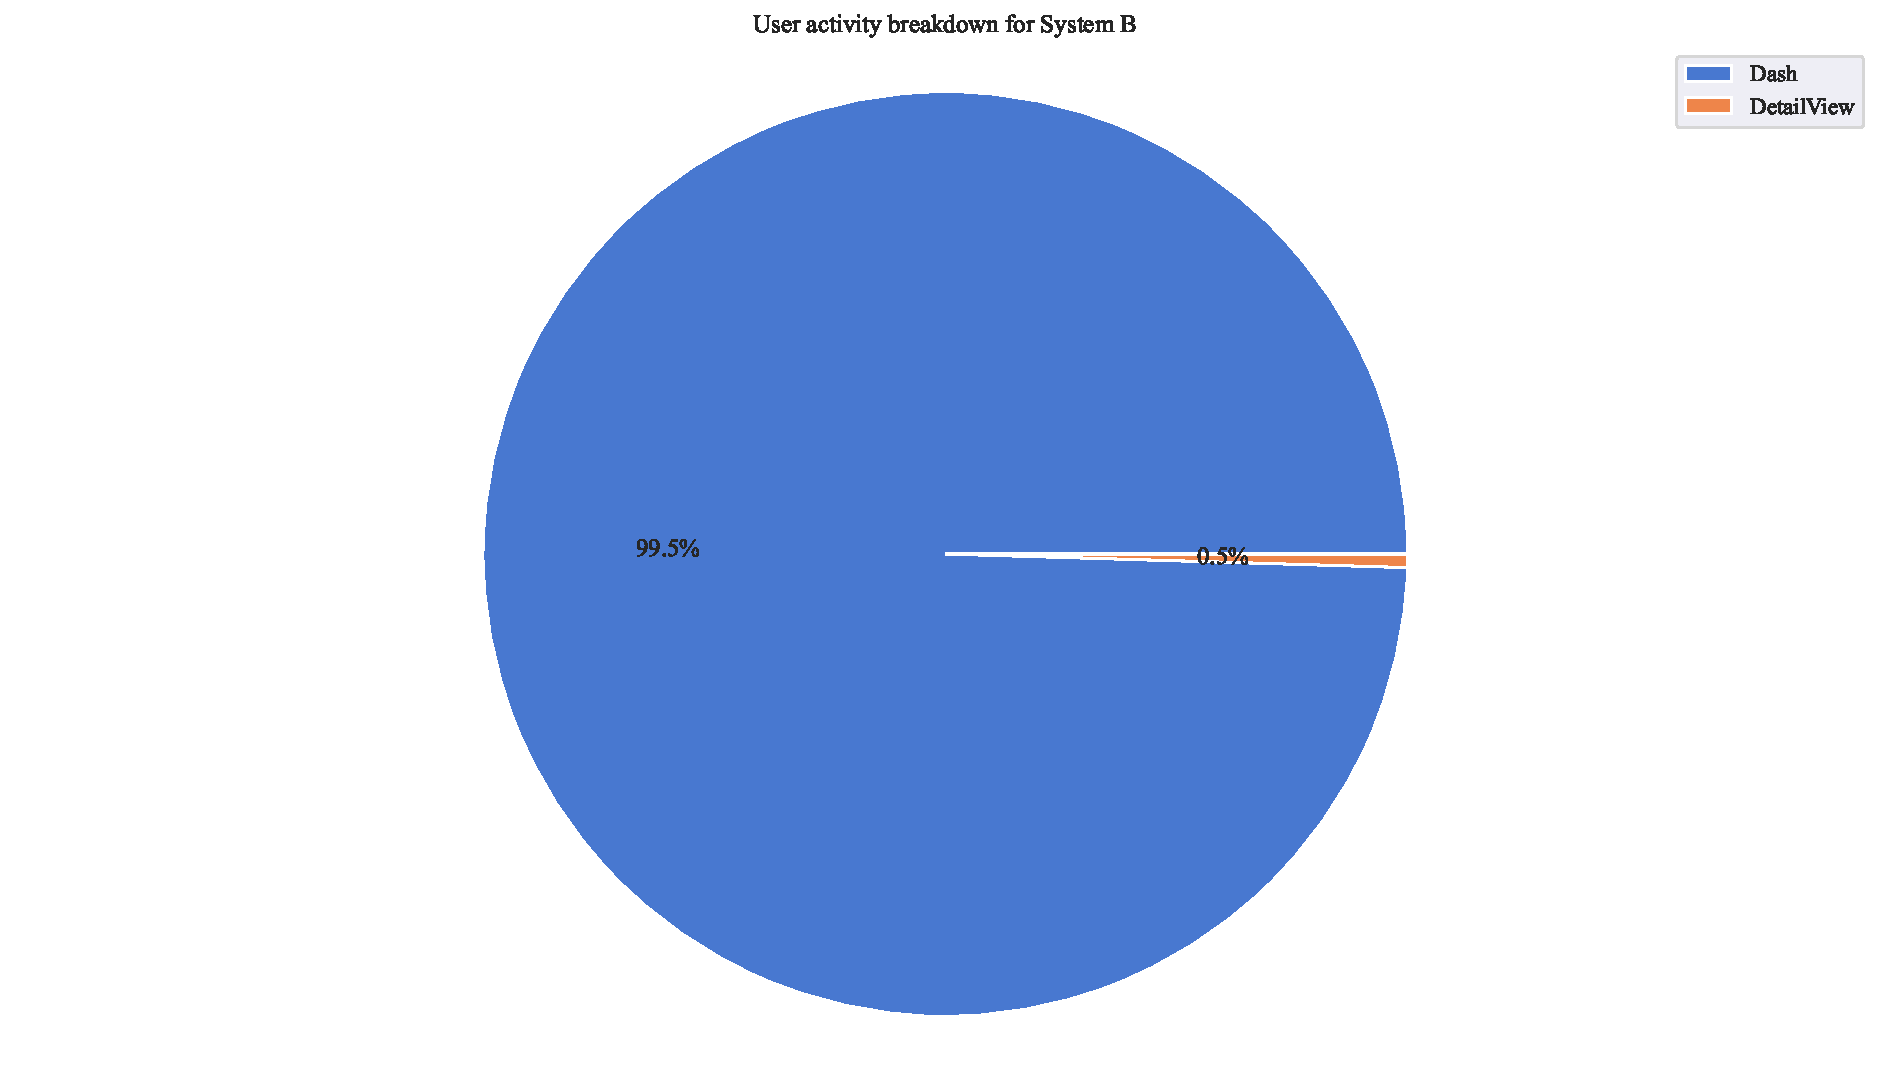
\includegraphics[width=0.95\linewidth]{img/ch3/analysis/case_B_breakdown.pdf}
	\caption[User activity types breakdown of System B]
	{\textit{User activity types breakdown of System B}}\label{fig:ch3_caseBBreakdown}
\end{figure}

In \Cref{fig:ch3_caseBBreakdown} the \texttt{Dash} user activity type is about $99.5\%$ of all recorded user activities. System B has fewer subsystems that require the user to interact with the web page to add data. The system mostly has web pages that display data only for the user. There weren't any \texttt{Report} user activity types as the users didn't create any reports to export from these subsystems.

\subsubsection{Maintenance prioritisation}
The maintenance prioritisation factor for the upper quartile user activities of the subsystem for case study B is calculated in \Cref{tbl:apx_caseB}.


    \begin{xltabular}{\textwidth}{XXXXX}
        \caption[Case study B's upper quartile maintenance pefromance]
        {\textit{Case study B's upper quartile maintenance pefromance}}
        \label{tbl:apx_caseB} \\
        \toprule
         \thead{$S_{X}$} & \thead{$P_N$}  & \thead{$A_N$} & \thead{$M_{PF}$} & \thead{$P_{R}$} \\
        \midrule
        \endfirsthead

        \multicolumn{5}{c}
        {\tablename\ \thetable{} -- continued from previous page} \\
        \midrule
        \thead{$S_{X}$} & \thead{$P_N$}  & \thead{$A_N$} & \thead{$M_{PF}$} & \thead{$P_{R}$} \\
        \midrule
        \endhead

        \midrule
        \multicolumn{5}{r}{{Continued on next page}} \\ \midrule
        \endfoot
        \endlastfoot
    \rowcolor{lightgray} $S_{417}$ & 1.0000 & 1.0000 & 1.0000 & 1 \\ 
  $S_{288}$ & 0.6756 & 0.3347 & 0.2261 & 2 \\ 
 \rowcolor{lightgray} $S_{258}$ & 0.9733 & 0.1663 & 0.1619 & 3 \\ 
  $S_{259}$ & 0.9733 & 0.1487 & 0.1448 & 4 \\ 
 \rowcolor{lightgray} $S_{170}$ & 0.7600 & 0.1487 & 0.1130 & 5 \\ 
  $S_{225}$ & 0.6089 & 0.1403 & 0.0855 & 6 \\ 
 \rowcolor{lightgray} $S_{72}$ & 0.6711 & 0.0780 & 0.0523 & 7 \\ 
  $S_{83}$ & 0.6711 & 0.0664 & 0.0445 & 8 \\ 
 \rowcolor{lightgray} $S_{268}$ & 0.5067 & 0.0720 & 0.0365 & 9 \\ 
  $S_{718}$ & 0.0089 & 0.0988 & 0.0009 & 10 \\ 
 \rowcolor{lightgray} $S_{409}$ & 0.0000 & 0.3774 & 0.0000 & 11 \\
        \bottomrule
    \end{xltabular}
    

The upper quartile of the maintenance performance of the subsystems of \Cref{tbl:apx_projectB_Normilised} are used to create the results of \Cref{tbl:apx_projectB_Normilised} using \Cref{eq:ch2_eventNormalised,eq:ch2_maintenanceFactorSimplified,eq:ch2_priorityNormalised}. The results of \Cref{tbl:apx_caseB} are visually presented in \Cref{fig:ch3_systemsBBar}.

\begin{figure}[!htb]
	\centering % cent the figure
	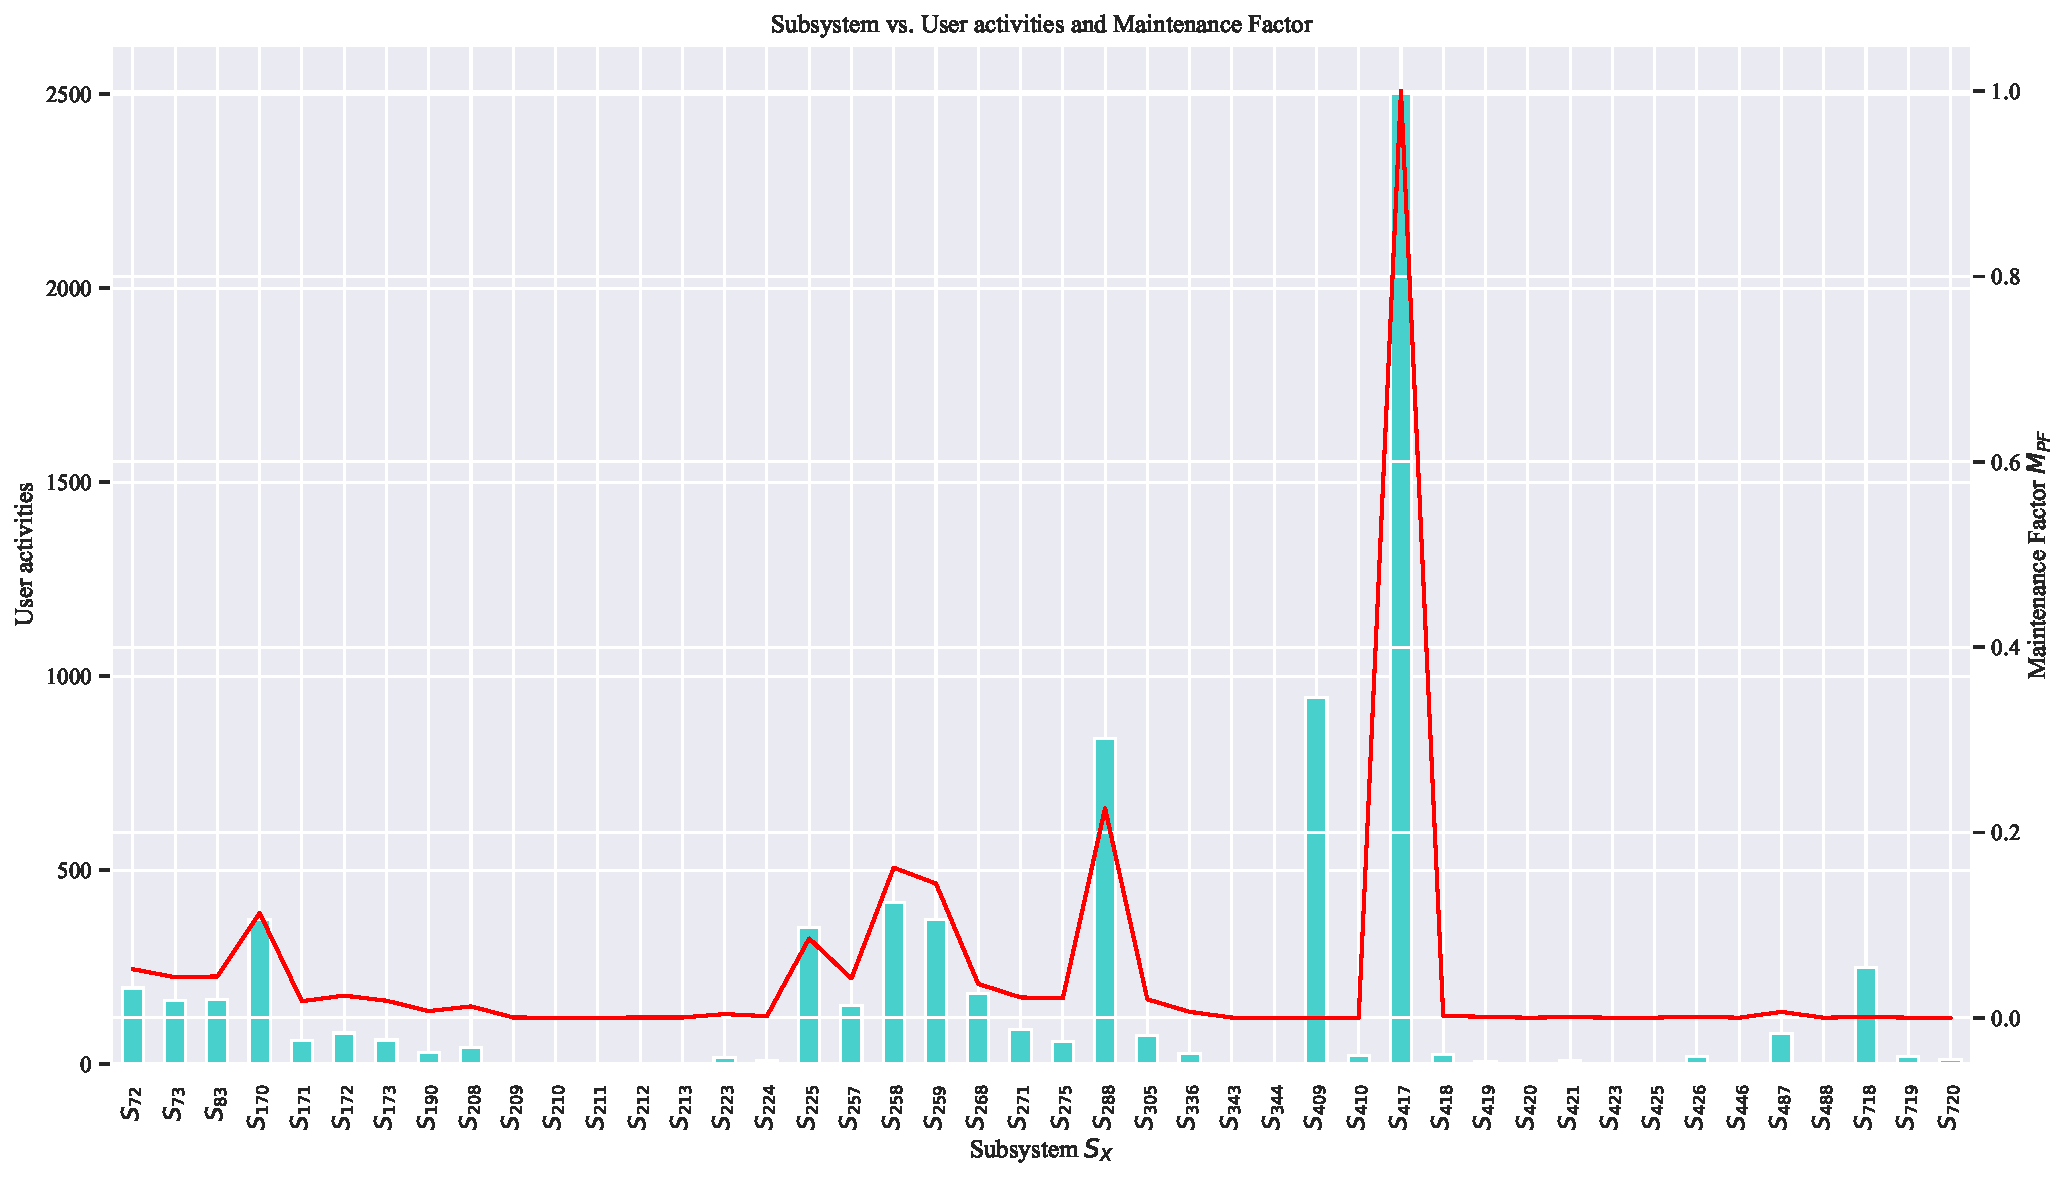
\includegraphics[width=0.95\linewidth]{img/ch3/analysis/case_B_subsystems_1.pdf}
	\caption[Maintenance performance calculation for system B]
	{\textit{Maintenance performance calculation for system B}}\label{fig:ch3_systemsBBar}
\end{figure} 

In \Cref{fig:ch3_systemsBBar} all of the subsystems have the majority \texttt{Dash} user activity type. About $99.5\%$ of the user activities is \texttt{Dash} user activity. This is due to that this older system made in \texttt{PHP} is only used for monitoring energy systems. The subsystems have simple inputs such as date pickers and category pickers for data. These type of inputs only refreshes the page which causes the more \texttt{Dash} activities to load new data for the user.\par $S_{417}$ has the most user activities, almost $2.5$ times higher than the second system $S_{409}$ and has the most users being active on this system. The number of user activities significantly decreases with the lower priority rank.

\clearpage

\subsection{Case study C results}
System C is also a \texttt{APS.NET Core Web SDK} software system. The software system has 7 primary user activity types that are described in \Cref{tbl:ch3_systemCActivityTypes}.

\begin{table}[!htb]
	\centering
	\caption[System A activity types]{\textit{System C activity types}}
	\label{tbl:ch3_systemCActivityTypes}
	\begin{tabularx}{\textwidth}{|l|l|X|}
		\hline \textbf{Activity} & \textbf{Functional requirement} & \textbf{Description} \\
		\hline \texttt{MenuAccessed} & \ref{fr:uatType1} & \RaggedRight This activity type is for when a user has navigated to a certain subsystem. \\ 
		\hline \texttt{HTMLElement} & \ref{fr:uatType3} & \RaggedRight This general activity type is for all other activities that the user initiates that send \textit{HTTP request} back to the server. This user type primarily is associated with HTML elements that the user used to interact with the subsystem. The sub-user activities of this primary user activity type are: \begin{itemize}
			\item SpanClicked,
			\item ButtonClicked, 
			\item DivClicked, 
			\item HyperLinkClicked,
			\item ListClicked, 
			\item LabelClicked, 
			\item ImageClicked, 
			\item FormInput, 
			\item SelectClicked
		\end{itemize} \\
		\hline \texttt{CustomControls} & \ref{fr:uatType3} & \RaggedRight System C has some custom-made HTML elements that have the same functionality as the \texttt{HTMLElement} user activity type. \\ 
		\hline \texttt{LoginAttempt} & \ref{fr:uatType2} & \RaggedRight This is a user activity for a log-out attempt by the user using the logout options available in the system to end their session. \\ 
		\hline \texttt{LogoutAttempt} & \ref{fr:uatType2} & \RaggedRight This is a user activity when the user uses any of the log-in page controls. \\
		\hline \texttt{ResetPassword} & \ref{fr:uatType2} & \RaggedRight This is a user activity when the user uses any of the reset password page controls. \\
		\hline \texttt{SessionTracking} & \ref{fr:uatType2} & \RaggedRight System C has some data stored in their session. Any changes to this data are tracked when the user interacts with any controls on the web page to change certain session data. \\
		\hline
	\end{tabularx}
\end{table}

For System C, the user activities listed in Table \ref{tbl:ch3_systemCActivityTypes} have been expanded to include the captured HTML elements that the users interacted with. As stated in Table \ref{tbl:ch3_caseStudies}, System C is an administrative software system used for configuring and managing Systems A and B. Compared to the monitoring software subsystems of Systems A and B, the user interaction in System C involves more complex user interactions.\par To facilitate analysis for the maintenance prioritisation the increased user activity types in Table \ref{tbl:ch3_systemCActivityTypes} can be grouped. The \texttt{HTMLElement} type is a grouped user activity type of the smaller individual user activity types. Despite their differences, these activity types share a common base functionality where it primarily shows the users' engagement with the system.\par System C uses a single logging point at the server side to capture the user event logs. The logging point for this implementation of the logging mechanism makes use of an action filter to:

\begin{itemize}
	\item ensures that the logging point is executed before the rest of the request is serviced by the function that is called by the subsystem,
	\item globally defined for all the controllers for the system,
	\item capture any additional user activity attributes,
	\item save the completed log into the database before the logging process is finally terminated.
\end{itemize}

This logging point is similar to the one used for system A but differs only in the key logging attributes that it needs to capture. Due to the HTML element's tag name used to define some of the user activities of \Cref{tbl:ch3_systemCActivityTypes}, the client side uses a similar logging point to capture the HTML element that the user interacted with.\par The client-side logging point adds the last or clicked HTML element that the user used for the user-based event and saves it in a custom request header. \Cref{fig:ch3_caseCBreakdown} is the user activity breakdown of the system C's activity types in \Cref{tbl:ch3_systemCActivityTypes}.

\begin{figure}[!htb]
	\centering % cent the figure
	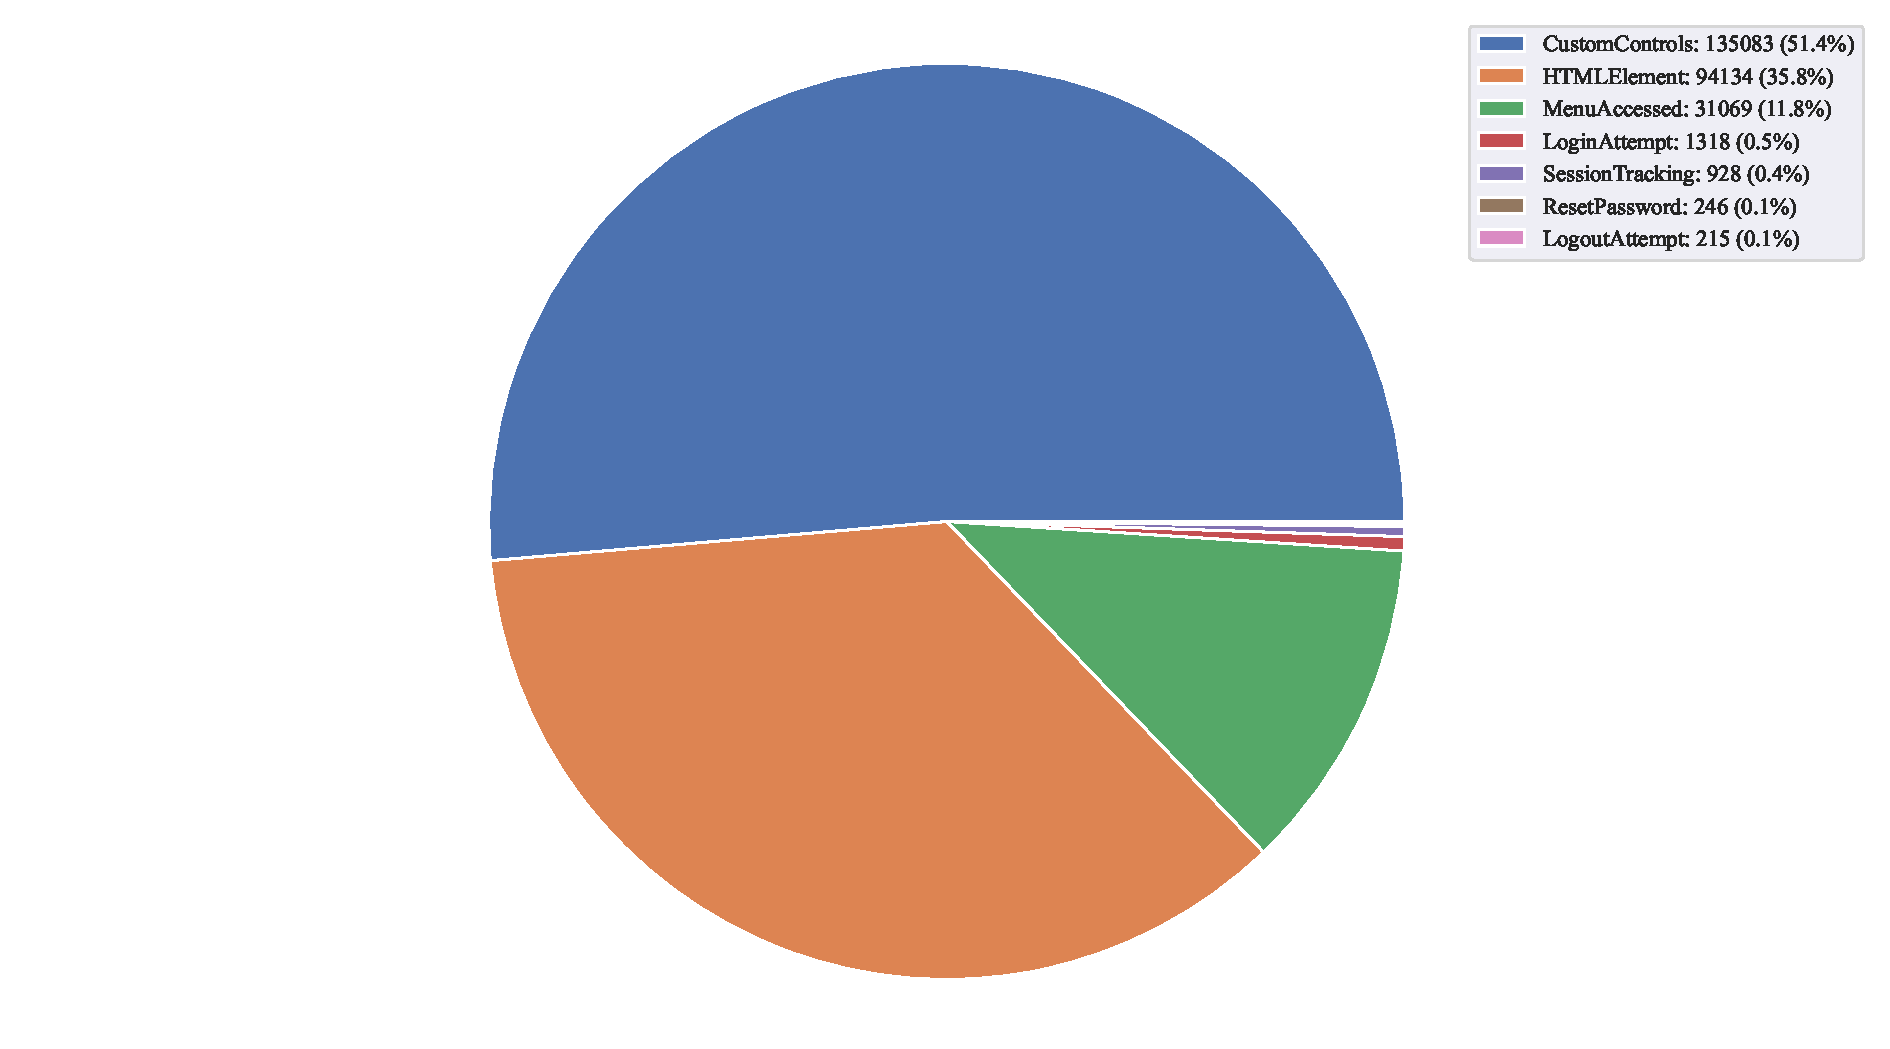
\includegraphics[width=0.95\linewidth]{img/ch3/analysis/case_C_breakdown.pdf}
	\caption[Case study 1 subsystem activities part 1]
	{\textit{Case study 1 subsystem activities part 1}}\label{fig:ch3_caseCBreakdown}
\end{figure}

\clearpage

The user activity breakdown in \Cref{fig:ch3_caseCBreakdown} the majority of the user activities for system C is \texttt{CustomControl} user activity type. The more interaction with the system increases the total amount of the general user activity types (\texttt{CustomControl} and \texttt{HTMLElement}).

\subsubsection{Maintenance prioritisation}
The maintenance prioritisation factor for the upper quartile user activities of the subsystem for case study C is calculated in \Cref{tbl:apx_caseC}.


    \begin{xltabular}{\textwidth}{XPPPP}
        \caption[Case study C's upper quartile maintenance pefromance]
        {\textit{Case study C's upper quartile maintenance pefromance}}
        \label{tbl:apx_caseC} \\
        \toprule
         \thead{$S_{X}$} & \thead{$P_N$}  & \thead{$A_N$} & \thead{$M_{PF}$} & \thead{$P_{R}$} \\
        \midrule
        \endfirsthead

        \caption[]{\continueCaption} \\
        \toprule
        \thead{$S_{X}$} & \thead{$P_N$}  & \thead{$A_N$} & \thead{$M_{PF}$} & \thead{$P_{R}$} \\
        \midrule
        \endhead

        \midrule
        \multicolumn{5}{r}{\continueText} \\ 
        \endfoot
        \endlastfoot
    \rowcolor{lightgray} $S_{97}$ & 1.0000 & 1.0000 & 1.0000 & 1 \\ 
  $S_{93}$ & 0.9931 & 0.8464 & 0.8405 & 2 \\ 
 \rowcolor{lightgray} $S_{12}$ & 0.5903 & 0.1694 & 0.1000 & 3 \\ 
  $S_{8}$ & 0.5625 & 0.1763 & 0.0992 & 4 \\ 
 \rowcolor{lightgray} $S_{5}$ & 0.2917 & 0.3312 & 0.0966 & 5 \\ 
  $S_{6}$ & 0.7083 & 0.0859 & 0.0608 & 6 \\ 
 \rowcolor{lightgray} $S_{1}$ & 0.8681 & 0.0660 & 0.0573 & 7 \\ 
  $S_{82}$ & 0.8681 & 0.0291 & 0.0253 & 8 \\ 
 \rowcolor{lightgray} $S_{14}$ & 0.5208 & 0.0391 & 0.0204 & 9 \\ 
  $S_{90}$ & 0.7778 & 0.0231 & 0.0180 & 10 \\ 
 \rowcolor{lightgray} $S_{13}$ & 0.3264 & 0.0529 & 0.0173 & 11 \\ 
  $S_{92}$ & 0.1736 & 0.0359 & 0.0062 & 12 \\ 
 \rowcolor{lightgray} $S_{11}$ & 0.2500 & 0.0223 & 0.0056 & 13 \\ 
  $S_{10}$ & 0.2778 & 0.0188 & 0.0052 & 14 \\ 
 \rowcolor{lightgray} $S_{46}$ & 0.4167 & 0.0095 & 0.0039 & 15 \\ 
  $S_{67}$ & 0.1181 & 0.0194 & 0.0023 & 16 \\ 
 \rowcolor{lightgray} $S_{7}$ & 0.2778 & 0.0070 & 0.0019 & 17 \\ 
  $S_{70}$ & 0.0833 & 0.0197 & 0.0016 & 18 \\ 
 \rowcolor{lightgray} $S_{95}$ & 0.1597 & 0.0076 & 0.0012 & 19 \\ 
  $S_{39}$ & 0.0417 & 0.0238 & 0.0010 & 20 \\ 
 \rowcolor{lightgray} $S_{79}$ & 0.0347 & 0.0182 & 0.0006 & 21 \\ 
  $S_{64}$ & 0.0625 & 0.0100 & 0.0006 & 22 \\ 
 \rowcolor{lightgray} $S_{51}$ & 0.0208 & 0.0245 & 0.0005 & 23 \\ 
  $S_{54}$ & 0.0486 & 0.0056 & 0.0003 & 24 \\ 
 \rowcolor{lightgray} $S_{30}$ & 0.0278 & 0.0077 & 0.0002 & 25 \\
        \bottomrule
    \end{xltabular}
    

The upper quartile of the maintenance performance of the subsystems of \Cref{tbl:apx_projectC_Normilised} are used to create the results of \Cref{tbl:apx_projectC_Normilised} using \Cref{eq:ch2_eventNormalised,eq:ch2_maintenanceFactorSimplified,eq:ch2_priorityNormalised}. The results of \Cref{tbl:apx_caseC} are visually presented in \Cref{fig:ch3_systemCBar}.

\clearpage

\begin{figure}[!htb]
	\centering % cent the figure
	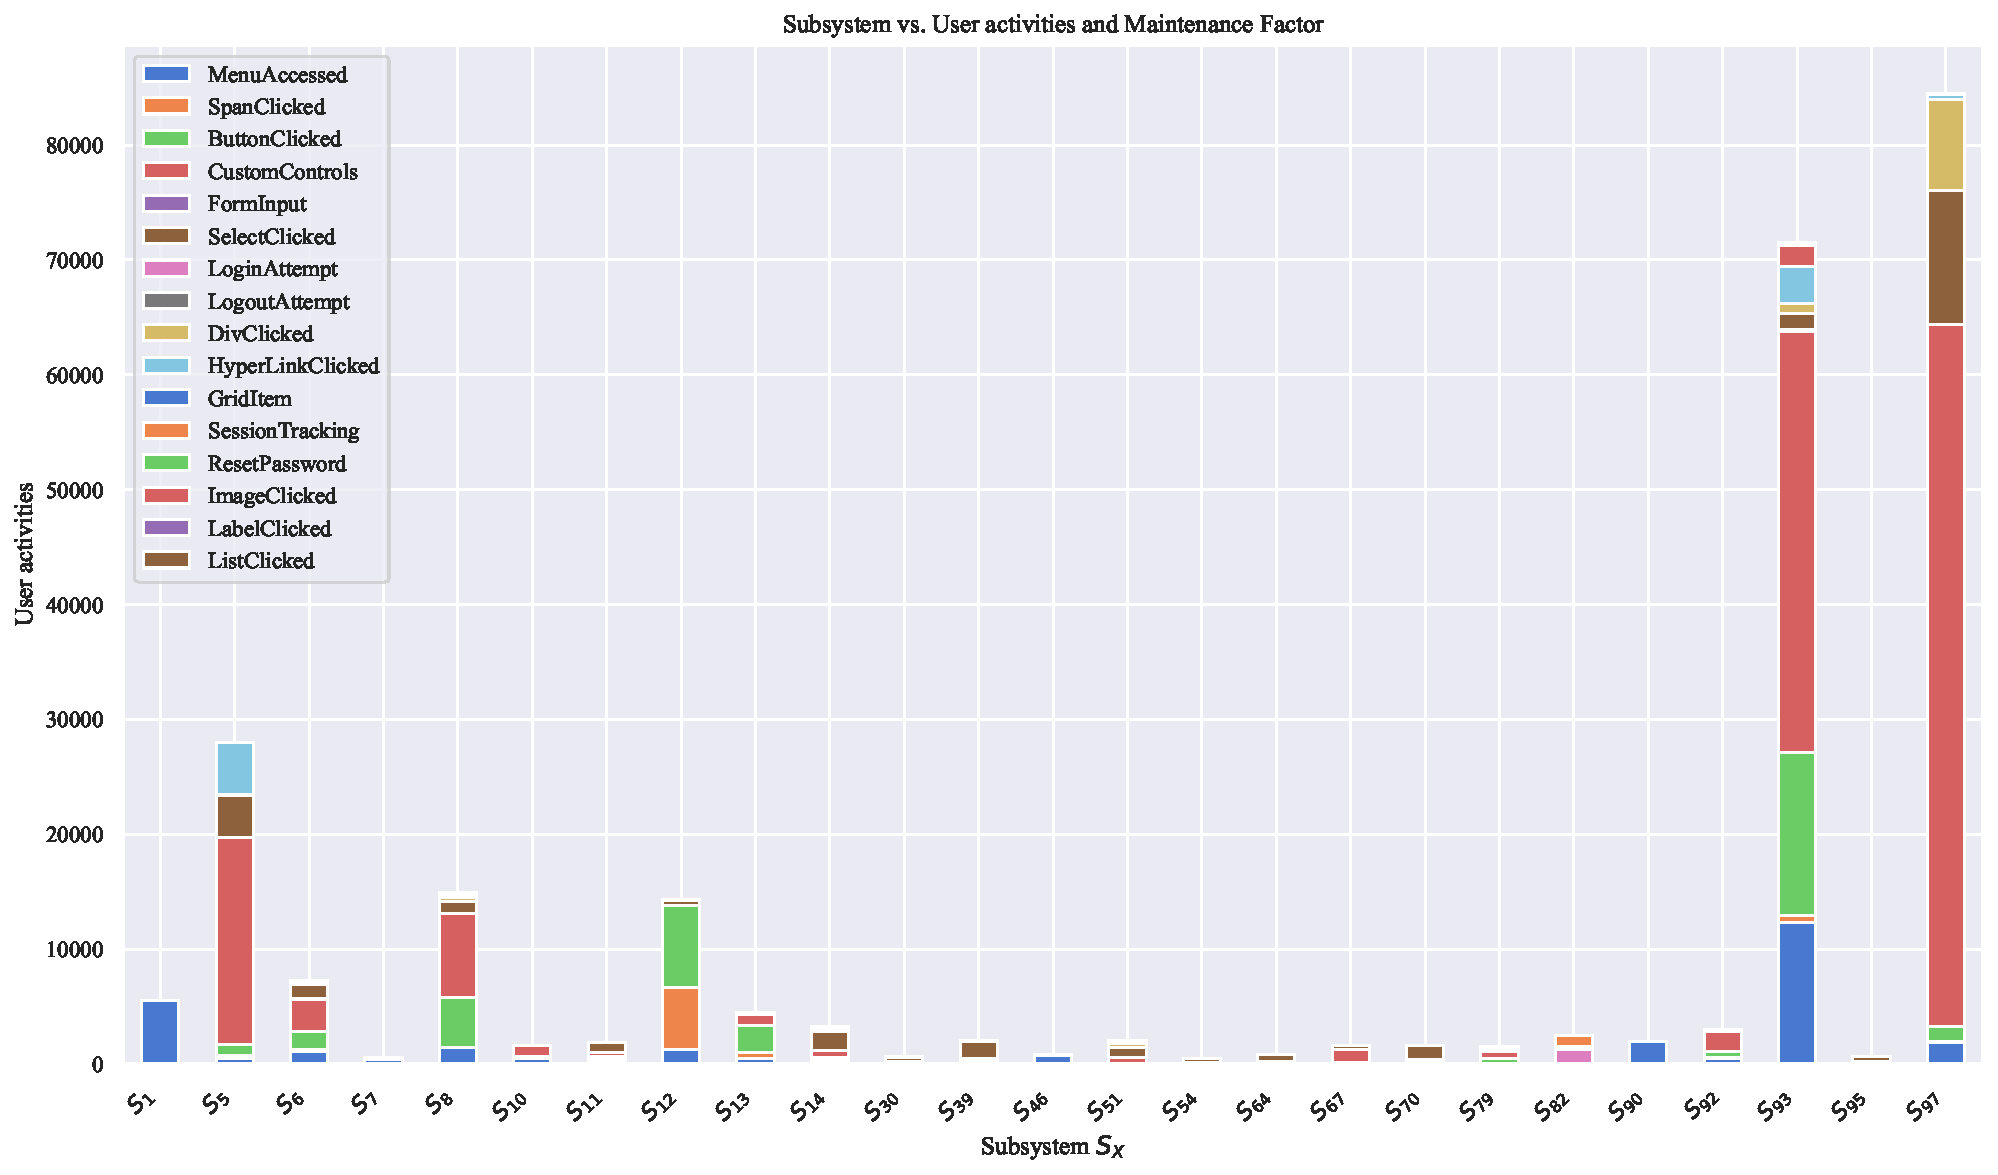
\includegraphics[width=0.95\linewidth]{img/ch3/analysis/case_C_subsystems_1.pdf}
	\caption[Maintenance performance calculation for system B]
	{\textit{Maintenance performance calculation for system B}}\label{fig:ch3_systemCBar}
\end{figure} 

In \Cref{fig:ch3_systemCBar} the top three subsystems ($S_{97}$, $S_{93}$ and $S_{12}$) majority user actvities are from general activity types. The high usage of these subsystems with a high amount of users linked to each one of them increased their maintenance priority factor. Other systems such as $S_{6}$, $S_{1}$ and $S_{82}$ have a higher priority normalisation than $S_{12}$ but have a significantly lower user activity normalisation. 

\subsection{Critical analysis results}

\section{Conclusion}